\documentclass[journal]{IEEEtran}
\usepackage{times}

% numbers option provides compact numerical references in the text. 

\usepackage{graphics} % for pdf, bitmapped graphics files
\usepackage{epsfig} % for postscript graphics files
%\usepackage{mathptmx}
%\usepackage{newtxtext}
%\usepackage{newtxmath}
\usepackage{times} % assumes new font selection scheme installed
\usepackage{amsmath} % assumes amsmath package installed
\usepackage{amssymb}  % assumes amsmath package installed
\usepackage{amsthm}
\usepackage{mathtools}
\usepackage{bm}
\usepackage{mathrsfs}
\usepackage{xcolor}
\usepackage{cite}
\usepackage{threeparttable}
\usepackage{multirow}
\usepackage{bigdelim}
\usepackage{algorithm}
\usepackage{algorithmicx}
\usepackage{algpseudocode}
\usepackage{graphicx}
\usepackage{subfigure}
\usepackage{comment}
\usepackage{pifont}
\usepackage{mnsymbol}

\usepackage{amsmath}

\usepackage[numbers]{natbib}
\usepackage{multicol}
\usepackage[bookmarks=true]{hyperref}

%\usepackage[toc,page]{appendix}

\newtheorem{theorem}{Theorem}
\newtheorem{definition}[theorem]{Definition}
\newtheorem{lemma}[theorem]{Lemma}
\newtheorem{corollary}[theorem]{Corollary}
\newtheorem{proposition}[theorem]{Proposition}
\newtheorem{remark}[theorem]{Remark}

%\pdfinfo{
%  /Author (Homer Simpson)
%   /Title  (Robots: Our new overlords)
%  /CreationDate (D:20101201120000)
%   /Subject (Robots)
%   /Keywords (Robots;Overlords)
%}

\begin{document}

\title{An Improved Maximal Continuity Graph Solver for Non-repetitive Manipulator Coverage Path Planning}

\author{Tong Yang, Jaime Valls Miro, Yue Wang$^*$ and Rong Xiong
\thanks{$^1$ Tong Yang, Yue Wang and Rong Xiong are with the State Key 
Laboratory of Industrial Control and Technology, Zhejiang University, P.R. China. 
}
\thanks{$^2$ Jaime Valls Miro is with the Robotics Institute at the University of Technology Sydney (UTS:RI), Sydney, Australia.}
\thanks{$^*$ Corresponding Author. \newline \indent
E-mail address: {\tt\small wangyue@iipc.zju.edu.cn}}
}

\maketitle

\begin{abstract}
A provable computational improvement to the problem of maximal continuity during non-repetitive object coverage with non-redundant manipulators is proposed in this work, where the physical meaning of optimality translates to the minimal number of end-effector lift-offs. Existing solutions enumerate each point on the surface with multiple ``colours'' according to the joint-configuration adopted, and model the problem as a painting problem of a graph with $M$ topological cells (a fully-connected section of end-effector points that can be painted with the same set of possible colours) and $N$ topological edges
(indicating the different choices of colour available). 
These works have proven that all optimal solutions can be collected in a finite number of steps. However, the solution grows exponentially in the size of $M, N$, becoming potentially intractable even for relatively simple graphs.
The proposed solution aims to avoid the need to enumerate all 
the edges by exploiting a topological invariance observed at colour intersections: 
the solution of an intersection-free graph can be uniquely represented by the colour of its boundary cells (in order), while enumerating internal edges and cells 
are shown to make no difference to the optimality of the solution, and can be safely omitted. 
A novel strategy is thus proposed to separate the graph into intersection-free sub-graphs.  
After enumerating and combining the solutions to each sub-graph to form the set of all optimal solutions, 
the complexity is proven to be reduced by a factor of $2^N$. Challenging scenarios are presented to validate the computational advantage of the proposed strategy.
\end{abstract}

\begin{IEEEkeywords}
Optimal Cellular Decomposition, Manipulator Coverage Task
\end{IEEEkeywords}

\IEEEpeerreviewmaketitle

\section{Introduction and Related Work}
\label{section_introduction}
The work in this manuscript is motivated by the non-revisiting coverage path planning (NCPP) along the surface of an object~\cite{Paul2013Novel}~\cite{Bhatt2019Concurrent} with a non-redundant manipulator, as illustrated by~Fig.~\ref{fig:toy_coverage_example}. 
Given the object's surface, the manipulator, 
the surrounding obstacles in the workcell and their related poses, for each reachable point on the surface there exist a finite number of inverse kinematic solutions in the manipulator configuration space, an example of which is depicted by the example mapping provided in~Fig.~\ref{fig:toy_coverage_graph_example}, left. 
Disregarding singular configurations~\cite{Yoshikawa1990Translational}, the collection of all valid configurations form disjoint sets in joint-space. When the manipulator transits from one set to another, it adopts a new pose altogether whereby the end-effector cannot remain on the object, being forcibly detached from the surface. This is an undesirable effect for tasks where smoothness and continuity are critical such as painting~\cite{li2011painting}, deburring~\cite{xie2016grinding}, welding~\cite{lee2011optimal}, scanning~\cite{Giataganas2013Cooperative} etc. 
In these instances, the desired solution translates to designing manipulator trajectories such that the end-effector visits each point on the surface exactly one time, whilst ensuring a minimum number of transitions between joint-space sets, or lift-offs. 

\begin{figure}[t]
\centering
\subfigure[Coverage illustration of a planar rectangular region with a non-redundant manipulator, depicting s(houlder)-l(eft)\&w(rist)-f(lipped), s-r(ight)\&w-u(nflipped), s-r\&w-f, and s-l\&w-u configurations. The transition between any pair imposes the adoption of a singular configuration thus preventing continuous traversability and a manipulator lift-off from the surface. By representing disconnectable manipulator configurations as different colours, an abstract topological graph with task-space colour distributions can be constructed as shown in (b) below.]{
	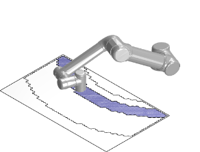
\includegraphics[width = 0.23\columnwidth]{figures/tmech_figures/slwf}
	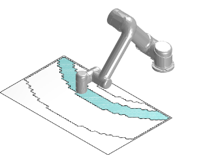
\includegraphics[width = 0.23\columnwidth]{figures/tmech_figures/srwu}
	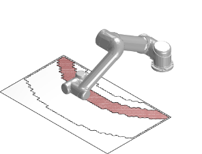
\includegraphics[width = 0.23\columnwidth]{figures/tmech_figures/srwf}
	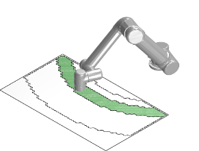
\includegraphics[width = 0.23\columnwidth]{figures/tmech_figures/slwu}
	\label{fig:toy_coverage_example}
}
\subfigure[Valid robot configurations form disjoint sets in joint-space, while their task-space FK mapping images (end-effector poses) may overlap. 
In the example, which for simplicity is illustrated with cells that are maximally $2$-overlapped, 
the resulting task-space graph conveys $N = 11$ undetermined edges constructed as shown by the dashed lines, thus separating the graph into $M = 11$ cells.
To facilitate the understanding whilst limiting clutter in the graph, 3 cells and 2 edges ($i$ and $j$ in dashed blue-green and blue-red respectively) are singled out. 
Solving the NCPP problem for the set of edges in the example can easily reveal all the optimal solutions in this case (two, depicted), demarcating the minimal bound for lift-offs as four. 
It is easy to appreciate how as more colours ``intersect", the algorithmic complexity to find the optimal solutions will soon escalate (more intricate examples are provided in Section~\ref{section_experiment}). It is also intuitive that should the green colour remain a complete set, both the red and blue colour cells would be split into further disconnected parts, 
leading to extra lift-offs. This hints at the fact ``intersecting" colours can be exploited to reduce the complexity of the solution.]{
	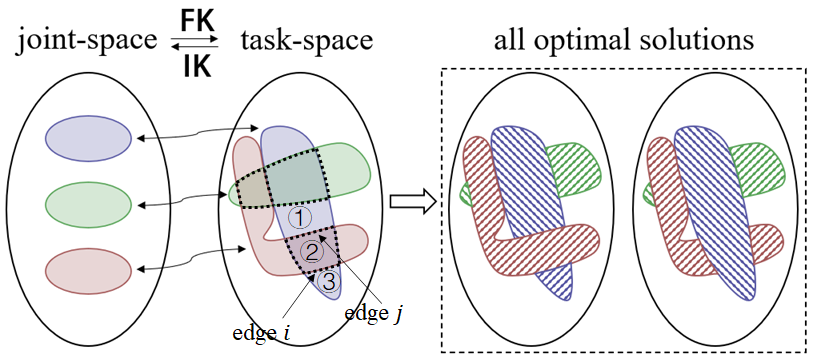
\includegraphics[width = 0.97\columnwidth]{figures/mapping_2}
	\label{fig:toy_coverage_graph_example}
}
\caption{A toy illustration of the problem arising when planning optimal non-revisiting coverage paths with a manipulator: (a) non-revisiting coverage of an object is dictated by the 
available configurations the manipulator can adopt. This leads to (b) disjoint sets in task-space, which conform the input to the NCPP problem. The optimal slicing of these sets leads to minimal discontinuities in tracing the surface with the end-effector. (Please note the above separate examples are independently chosen to best illustrate the problem and do not correspond to each other).
}
\label{fig:mapping}
\end{figure}

\begin{comment}
\begin{figure}[t]
\centering
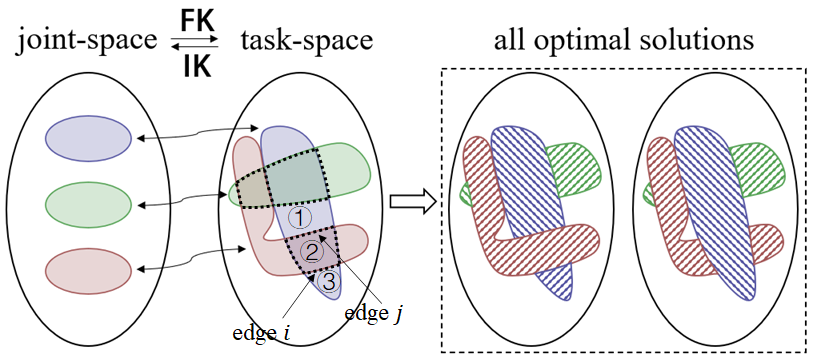
\includegraphics[width = 0.48\textwidth]{figures/mapping_2}
\caption{A toy illustration of the problem arising when planning optimal non-revisiting coverage paths with a manipulator: valid robot configurations form disjoint sets in joint-space, while their task-space FK mapping images (end-effector poses) may overlap. 
In the example, which for simplicity is illustrated with cells that are maximally $2$-overlapped, the resulting task-space graph conveys $N = 11$ undetermined edges constructed as shown by the dashed lines, thus separating the graph into $M = 11$ cells.
To facilitate the understanding whilst limiting clutter in the graph, 3 cells and 2 edges ($i$ and $j$ in dashed blue-green and blue-red respectively) are singled out.
Solving the NCPP problem for the set of edges in the example can easily reveal all the optimal solutions in this case (two, depicted), demarcating the minimal bound for lift-offs as four. 
It is easy to appreciate how as more colours ``intersect", the algorithmic complexity to find the optimal solutions will soon escalate (more intricate examples are provided in Section~\ref{section_experiment}). 
It is also intuitive that should the green colour remain a complete set, both the red and blue colour cells would be split into further disconnected parts, leading to extra lift-offs. 
This hints at the fact ``intersecting" colours can be exploited to reduce the complexity of the solution.
}
\label{fig:mapping}
\end{figure}
\end{comment}


Early reports on the generic \textit{coverage path planning} (CPP) problem focused on geometric path designing~\cite{Kaljaca2020Coverage}~\cite{Oriolo2005Motion}, particularly for mobile platforms operating in planar surfaces, such as boustrophedon~\cite{choset1998coverage} or spiral paths~\cite{hassan2018a}. 
Additional strategies were later proposed that transformed the coverable region into smaller partitions, or \textit{cells}, where continuous coverage paths could be guaranteed. A body of novel partitioning \textit{cellular decomposition} strategies emerged~\cite{Acar2002Morse}~\cite{choset2000exact}~\cite{huang2001optimal}~\cite{Atkar2009Hierarchical}~\cite{Hassan2017Simultaneous}, applied directly onto the area to be covered. This is an ineffective strategy when transferred from task to joint space for manipulator planning since the kinematic mapping between the two spaces is non-bijective: as illustrated in Fig.~\ref{fig:mapping}, the forward kinematic relationship from the configuration space to the surface is surjective (many-to-one) and locally flat (one-to-one from each connected component of the valid configuration space to the surface). 
The problem is further compounded when the end-effector can only visit each point on task-space once, leading to numerous pose reconfigurations during the motion of the end-effector~\cite{rososhansky2011coverage}.
Many criteria in the classic CPP problems have been adapted to the manipulator NCPP task, such as time to completion~\cite{lu2020time} or energy consumption~\cite{mei2004energy}, and optimal mobile manipulator pose for a given coverage in task-space has also been investigated~\cite{paus2017a}~\cite{Fan2021Base}~\cite{Kalawoun2018Optimal}. However, optimising  end-effector lift-offs for increased smoothness and continuity has been rarely exploited. 
Recent propositions in the literature to tackle the problem decomposed the task-space area into a topological graph ensuring continuous joint-space coverage within each cell, and looked for solutions where maximal continuity between cells existed~\cite{Yang2020Cellular}, as intuitively depicted in Fig.~\ref{fig:mapping}. 
All maximal-continuous cellular decompositions were proven to be collectable in a finite number of steps, defined by edges that represent the smallest, inseparable elements and cells that could only have a finite number of different sub-divisions.  

\begin{figure}[t]
\centering
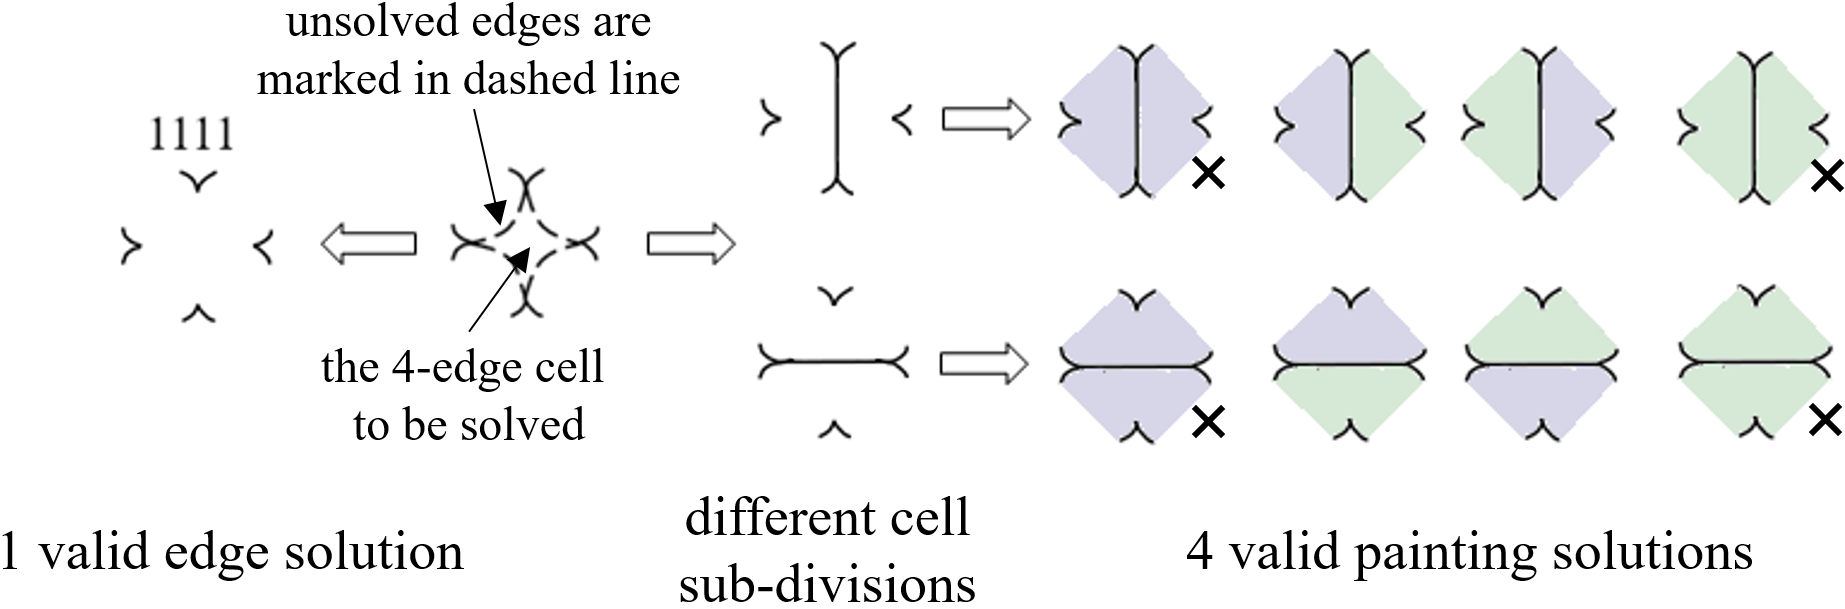
\includegraphics[width = 0.48\textwidth]{figures/many_to_one_3}
\caption{An illustration of the many-to-one relation between edge and painting solutions. 
Let a cell with $4$ adjacent cells (a $4$-edge cell) have 2 possible colours ``blue" and ``green", then $\alpha = 4, K = 2$. From the point of view of solving edges, the binary number $1111$ specifies one solution, but the corresponding valid painting solutions are multiple, $4$ to be precise: there are $E=2$ ways to divide the multi-edge cell into $3$-edge sub-cells, and $\alpha-2 = 2$ sub-cells are generated which can be filled with the $K (=2)$ possible colours. After enumerating $E\cdot K^{\max\{\alpha-2, 1\}}$ cases, four of them are removed (no subdivision when there is only one possible colour for all sub-cells), shown crossed-out, leaving the remaining four valid painting solutions.
}
\label{fig:many_to_one}
\end{figure}


This is however an intensely computational process, growing exponentially in the size of the graph
\footnote{For a better understanding of the ensuing terminology, the reader is referred to the preliminary definitions set out in Appendix.}.%~\ref{appendix_preliminaries}.}. 
 % <JVM> this could also be a footnote perhaps
Let there be $M$ topological cells and $N$ internal topological edges in the modelled graph to be solved. The number of edges for the $i$-th cell is $\alpha_i$, and denote the number of possible colours to fill cell $i$ as $K_i$.   
It has been shown how a binary array of length $\alpha_i$ can be used to index all possible different divisions of cell $i$~\cite{Yang2020Cellular}, whereby $0$ at a given position enforces the cell having a different color to its adjacent cell, whilst $1$ compels the same choice of colour. 
However, as supported by the illustrative example shown in Fig.~\ref{fig:many_to_one} for one of the edge solutions $(1111)$ and $2$ possible colours available for painting, the binary array does not uniquely represent a valid painting solution: the cell may be divided into two parts with differing colours, while each part themselves connect to their two adjacent cells. Following the cell sub-divisions, $4$ valid painting solutions of this cell appear corresponding to the edge solution $1111$. 



\begin{comment}
Since every edge has two adjacent cells, 
the relation of $\alpha_i$ to $N$ is established by
\begin{equation}
N = \frac{1}{2}(\sum\limits_{i=1}^M \alpha_i - \tilde{N})
\end{equation}
($\tilde{N}$ simply denotes the number of edges on the outer boundary of the graph, %(with adjacent cells $-1$ ) 
which are determined and thus need not be enumerated). 
%Note that, although proving the finiteness of dividing each cell into sub-cells is enough for proving the finiteness of the whole process, the overall algorithmic complexity is far more than $2^N$, 
It has been shown in the Fig.~\ref{fig:many_to_one} counterexample how there is no one-to-one correspondence between the edge and painting solutions. 
The edge solution depicted, 1111, could be painted with 4 different valid painting alternatives.
Generically \textcolor{red}{is this from Tmech? I think so, so we need to reference it, not just drop it expecting the reader will be able to figure that out, not possible!} it has been proven by the cell sub-division strategy described in~~\cite{Yang2020Cellular} how if $\alpha_i \geq 4$, cell $i$ will be iteratively divided into $(\alpha_i-2)$ $3$-edge sub-cells\footnote{Here for simplicity we only consider the worst case presented in~\cite{Yang2020Cellular}. Beyond dividing fully into $3$-edge cells, the complexity of enumerating other cell sub-divisions is omitted \textcolor{red}{but it is also part of the enumeration of edges, shouldn't we? or you mean that taking the worst case, 4 adjacent cells, represents the highest computation and therefore we only need to consider this case for complexity calculation? - which I agree with}.}, and each sub-cell can be individually assigned with $K_i$ colours. Let there be $E_i$ different ways to divide cell $i$ into sub-cells, the overall complexity %\footnote{Here we disregard speeding-up tricks proposed in existing literature, because they are also valid in the algorithm proposed in this work. } 
can then be calculated as
\end{comment}

There is a need to enumerate all the edges for each cell, leading to all different colours to be subsequently filled in to create all posissible solutions~\cite{Yang2020Cellular}. This is a costly exercise. For the more generic case of a multi-edge ($\alpha_i \geq 4$) cell, other than the simple case of considering it as a whole, it may be sub-divided into up to $(\alpha_i-2)$ sub-cells, and each sub-cell can be individually assigned with $K_i$ colours. Considering a worst case scenario, let there be $E_i$ different ways to divide cell $i$ into $(\alpha_i-2)$ sub-cells, then $E_i\cdot K_i^{\max\{\alpha_i-2, 1\}}\cdot 2^{\alpha_i}$ steps are required for a single cell. Iteratively enumerating each cell and noting that each edge will only be enumerated once in the process, the algorithmic complexity can be calculated as
\begin{equation}\label{equ:tmech_complexity}
\prod\limits_{i=1\atop\alpha_i \geq 4}^{M}E_i\cdot \prod\limits_{i = 1}^M K_i^{\max\{\alpha_i-2, 1\}} \cdot 2^N
\end{equation}


\begin{comment}
Also note that as a dual graph of the commonsense ``node-edge" graph, the cells, edges and vertices correspond to the nodes, edges and faces (temporarily denoted as $F$ which has no usage in the NCPP problem), respectively. Then the relation of the number of cells $M$ and the edges $N$ is given by the Euler's formula for planar graph, 
\begin{equation}
N-M = F-2
\end{equation}
In a complicated graph we must have $F\gg 2$, then $N \gg M$. 
\begin{color}{blue}
We observe that enumerating an edge is a too trivial process to lead to different topologies of the resulting solution. See Fig.~\ref{fig:mapping}, where if edge $i$ is kept, then $j$ need not be removed, because even if cell \ding{172} and \ding{173} are connected, it makes no difference to the topology if cell \ding{174} is not connected together. 
In other words, existing works have avoided equivalent cellular decompositions under the equivalence of continuous modification of the cutting paths of cells. But looking at the topology of the resulting solution from a top-down view might further avoid carrying out equivalent multi-step processes in enumerative solving. 
In this paper, we introduce a high-level abstraction of the topology, the \textit{intersection}, which is the origin of the multiplicity of the optimal solutions. We show that intersections are unavoidable and have to be enumeratively solved. 
However, by separating the graph into intersection-free sub-graphs, all intersections are implicitly enumerated while sub-graphs are combined. As a result, the algorithmic complexity of enumerating all edges, $2^N$, is removed. 
\end{color}
\end{comment}

\begin{figure}[t]
\centering
\subfigure[a cell-graph to be solved]{
	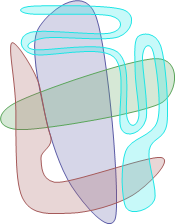
\includegraphics[width = 0.18\textwidth]{figures/cell_graph}
}
\subfigure[the node-graph]{
	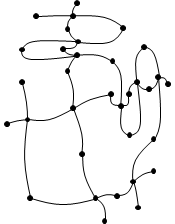
\includegraphics[width = 0.18\textwidth]{figures/node_graph}
}
\caption{Quantitive relationship between the cell-graph notation adopted in the manipulator coverage task and the traditional node-graph concepts in classic graph theory. In this example there are $33$ vertices, $39$ edges, and $8$ faces ($7$ cycles $+$ $1$ outer region reaching the infinity) in the node-graph, which correspond to $33$ cells and $39$ edges in the cell-graph. }
\label{fig:node_graph}
\end{figure}
% <Tong> this is a bit trivial, but it would read more nicely to show the above, as in  
% there are $33$ vertices (red), $39$ edges (green), and $8$ faces (blue)
% for instance ... not sure if the colour scheme will look niece, feel free to adopt another one ... but use "mild" colours, pastel-like, as per your figures in the paper, I like them, not bright red-green-blue ... infinity face can be done with a blurred border figure or similar? 
% <ty> I will upload two new figures to git
% <Tong> don't quite like them, I don't think they add clarity, perhaps the opposite is true. We leave as is, it is clear enough in my mind.

%\subsection{Contribution of This Paper}

Careful examination of the topological graph leads in this work to the introduction of a high-level abstraction, the \textit{topologcal intersection} which is the origin of the multiplicity of the optimal solutions. It is hereby proven that intersections are indeed unavoidable and have to be enumeratively solved. However, separating the graph into intersection-free sub-graphs leads to all intersections being implicitly enumerated when the sub-graphs are recombined later to calculate the final solutions. The end result is the removal of the substantial complexity in enumerating all edges, in the order of $2^N$. 

It should be noted that an assumption of simply-connected cells underlies the structure of the proposed solution. As it has already been 
proven~\cite{Yang2020Nonrevisiting} % <Tong> pls add ref (RSS20) <ty> fixed
that for graphs with multiply-connected cells, iterative enumeration can reduce the problem to that of a simply-connected cell graph, 
the proposed solver improvement is generic to any type of cell connectivity.


The significance of the algorithmic improvement can also be revealed by invoking the cell-graph notation promoted in this work and the traditional concept of node-graph in classic graph theory. This equivalence is pictorially shown in Fig.\ref{fig:node_graph}, whereby a one-to-one correspondence between the cells and edges in a cell-graph and the vertices and edges in a node-graph can be established. The Euler's formula~\cite{Bondy1976Graph} for planar graphs yields: 
\begin{equation}
V - E + F = 2
\end{equation}
where $V, E$, and $F$ are the number of vertices, edges, and faces in the node-graph, respectively. 
This relationship highlights the large number of edges in a cell-graph, $F-2$ greater than the number of cells: 
\begin{equation}
N - M = E - V = F - 2
\end{equation} 
It can be observed how in complicated graphs where $F$ will be necessarily large, reducing algorithmic complexity by $2^N$ represents a notable breakthrough. 
This relationship to classic graph theory also points towards a potential contribution in other related research areas besides the manipulator NCPP problem, which is beyond the scope of this work. 


The remainder of this paper is organised as follows. Section~\ref{section_intersection} introduces the concept of \textit{topological intersection} and the \textit{intersection-free graph} property.
Section~\ref{section_graph_separation} describes concrete steps to separate a graph into intersection-free sub-graphs. 
Solutions to these can then be combined to construct the optimal solutions for the full graph. 
Details about the complexity advantage in solving the problem following the proposed strategy are mathematically proven in Section~\ref{section_complexity}, whilst experimental results from simulations are collected in Section~\ref{section_experiment}. Final concluding remarks are gathered in Section~\ref{section_conclusion}.


\section{Optimality via ``Topological Intersections''}
\label{section_intersection}
In this section, we introduce a topological invariant variable, named \textit{intersection}.  
The enumeration of intersections will be shown to be the core element in the graph solver leading to notable inefficiencies when solving a full graph with intersections, versus solving an equivalent intersection-free graph. 

A topological invariant variable is a character of the given structure which is invariant under the admissible set of modifications to the structure, 
such as the connectedness of a region under homeomorphic mappings. A typical application of topological invariants in mathematics is for distinguishing two different objects: first the topological invariant is defined, then two objects can be shown to be different topological invariants, hence not equivalent 
under the modifications that preserve the topological invariant. 
However, unlike this mainstream usage of topological invariants, in this work the key observation is not leveraging intersections, but how to avoid intersections altogether. 

The methodology in this section aims at constructing ``counter-examples" that restrict the potential directions any algorithmic complexity 
improvements may take. As will be concluded, revealing all optimal solutions requires the complete set of intersections to be enumerated. Yet enumerating intersections increases the complexity of any solver by a multiplicative factor. 
%As such, all existing algorithms and any likely improvements to solve the graph may look for a ``bare" enumeration of intersections, instead of an implicit enumeration by enumerating all edges and cells. 
% <Tong> I like the way it reads below better. The introduction of the "implicit" term ( 'enumeration by enumerating all edges and cells') is in my opinion not clear at this point of the paper. My more generic explanation I feel does the same yet is more intuitive to understand I feel. Happy if you have another opinion, needs to be correct in the generic terms that I describe it of course, let me know if you think it does not. Otherwise we leave.   
% <ty> I think the current version is perfect. 
As such, existing algorithms and any likely improvements to solve the graph should note the ``explicit" reduction in the enumeration of intersections, and look for a minimalistic set of them to be solved.
In that regard, it makes the simplified representation adopted in this work of a wholly intersection-free graph apparent, and points towards an intersection-free graph separation scheme which ensures all intersections are placed at common boundaries of sub-graphs, presented in detail in Section~\ref{section_graph_separation}. 


\begin{comment}
The methodoly in this sections aims at constructing ``counter-examples" that reveal the inexistence of a possibly more efficient algorithm which avoids enumerating intersections. 
As will be concluded, the enumeration of intersections unavoidably leads to worse-off algorithmic complexity. 
As such, any likely improvements to solve the graph over other possible algorithms should note the ``explicit" reduction in the enumeration of intersections. In that regard, it makes the simplified representation adopted in this work of an intersection-free graph apparent, and points towards the intersection-free graph separation scheme proposed in Section~\ref{section_graph_separation}. 
\end{comment}


\begin{figure}[t]
\centering
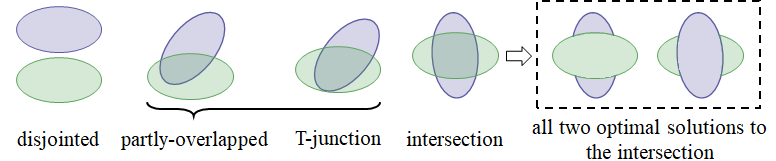
\includegraphics[width = 0.48\textwidth]{figures/basic_shape_3}
\caption{Illustration of the basic relationships between the reachable area for a two-colour case. In all but the intersection scenario, each colour can keep itself fully connected. T-junction can be seen as a special instance of the generic partly-overlapped case, as it can be transformed back to the generic case through continuously modifying the boundary of the colours. Only the intersected case needs solving, and it is apparent that the two optimal solutions are not topological equivalent: they have a different number of connected regions for each colour, depending on whether the blue or the green colour is chosen in the connecting area.}
% <Tong> the way I understand it, if correct, leave as is.
% I actually note that the "number" of connecting regions is the same though ...?
% <ty> It is correct. I simply add "for each colour" for clarity. 
\label{fig:basic_shape}
\end{figure}





\subsection{Definition of Intersection}
\begin{definition}
(Intersections) An intersection is a class of distribution, more concretely overlapping, of the coverable region of multiple colours, describing an inevitable interruption of the connectedness of one colour by other colours. 
\end{definition}
Denoting $\#\{\mbox{NCPP}(G)\}$ as the minimal number of end-effector lift-offs given the graph $G$, and 
$\#\{\mbox{CPP}(G)\}$ as that of the repetitive coverage path planning problem, the existence of intersections can be formally revealed by
\begin{equation}
\mbox{intersection exists}\Leftrightarrow \#\{\mbox{NCPP}(G)\} - \#\{\mbox{CPP}(G)\} > 0
\end{equation} 

% <Tong> I reworded the below a bit, I think I capture what you meant. I feel what you say is obvious, and I don't quite fully understand why it is here. 
% It is noteworthy, but why here in this Defintion 1 is not clear to me. I wonder if it may have a better place elsewhere?
% Unless something is wrong, I like how it is written. I'm just questioning why it follows Definition 1, which describes what an intersection is?
% <ty> I think the current version is perfect. After we enumerate one cell, if we say the process is equivalent to "removing other colours", the graph becomes as if it hasn't be enumerated. So after we note this, the intersection is well-defined in any partly-solved graph. 
In regards to intersections and graph solving it is worth noticing that painting the colour of one cell is equivalent to removing all the 
other possible colours it could be painted with. Hence, as a graph is being solved the distribution of coverable region by the different colours 
keeps changing, unconsciously leading to the possible elimination of some of the intersections. 
Generally, a graph to be solved admits intersections, whilst a solved graph where each cell only preserves one colour is % apparently <Tong> why apparently? it will be intersection-free, one colour per cell % <ty> It is apparent because there is no multi-colour cell, thus there is no overlapping between colours and obviously the connectedness of colours are independent with each other. But I think removing it is also correct. 
intersection-free. 
Reducing the number of intersections until none remains is the target of the graph solver.  

The invariance of intersections is revealed in the connectedness of cells: 

\begin{proposition}
\label{lemma:invariance}
(Invariance under homotopic cutting paths) In a (partly-solved) graph, any continuous modification of the cell cutting paths will not reduce the number of intersections in the graph. 
\end{proposition}
\begin{proof}
It has been shown in \textbf{Lemma}~\ref{lemma:tmech_equiv} that all cutting paths (and preserved edges) need not be intersected, hence the continuous modification of cutting paths will not change the connectivity of any cell. That means there will not be a case whereby two disconnected cells with the same colour become connected after continuous modification of cutting paths, nor a case that a single solved cell is truncated into two disconnected parts. Hence the intersections will be invariant. 
%There is certainty in the fact that the number of intersections in a partly-solved graph will not reduce under continuous modification of cell cutting paths. 
\end{proof}

Typically, for the simplest case, the coverable area of two colours may be fully disjointed, partly overlapped, or intersected, as shown in Fig.~\ref{fig:basic_shape}. It can be observed how colours can be kept connected in the disjointed and partly overlapped cases, but critically in the intersection case one colour being connected will truncate the other colour in two parts.

\begin{figure}[t]
\centering
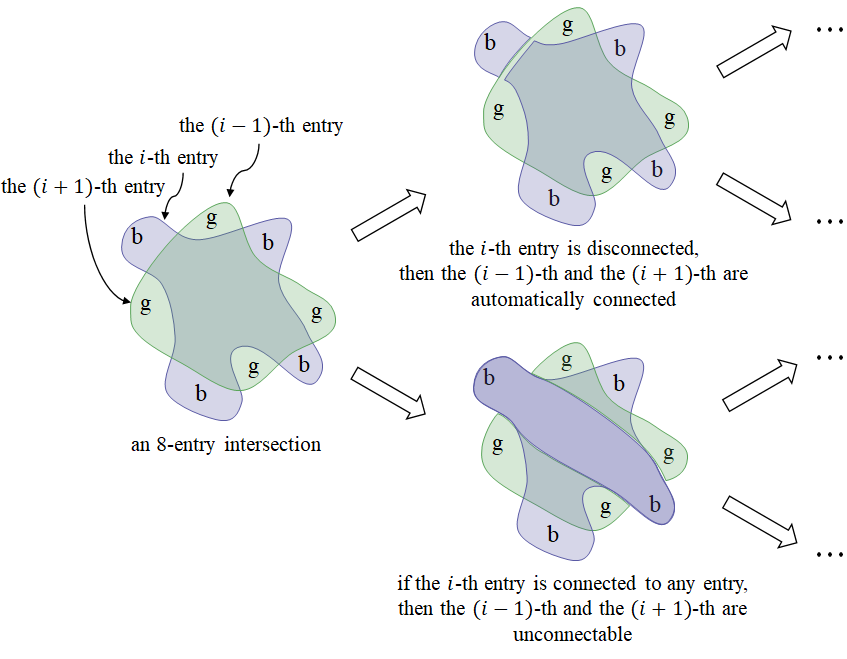
\includegraphics[width = 0.48\textwidth]{figures/new_multi_entry}
\caption{An example with an $8$-entry intersection is depicted on the left. The figure also illustrates the process of solving a single intersection with a simpler example where adjacent entry cells have been assigned % a unique <Tong> by definition, an entry HAS a unique colour, Def 3. The way this reads if as if it is a special case, it is not. I think the special case is that entries are alternate colours. I still fail to see the significance to be honest, I've rewritten what I thought was correct, pls check! ... 
% <ty> Now it is correct
alternate colours ``b(lue), g(reen), b, g, $\cdots$".  
It is apparent from the two token scenarios shown that an exhaustive enumeration will be required to obtain all optimal cellular decompositions.
% <Tong> the next phrase is a bit out of place, as we don't show all the connected regions, it is odd. However being here allows for it to be referred later it in Corollary 5, but you did not, see how I did. If correct, leave
% <ty> It is correct. It should be referred in txt. I have added them based on your comments. 
It will be established later in \textbf{Corollary}~\ref{coro:enum}) that given $n = 8$ entries, the minimum number of connected regions can be directly calculated as $5$.  %, while given the totally symmetric distribution of colours, 
 %It depicts the standard transformation whereby consecutive adjacent cells can be filled in same colour through shrinking the boundary of one of the colours, hence reducing to it can be transformed back to the normal case. 
}\label{fig:multi_entry}
\end{figure}

\subsection{Intersection Properties}
The intersection properties defined in this section represent a ``drawback" that limits the emergence of more efficient algorithms. 
Note that these pitfalls do not directly contribute to the algorithm design itself, but indicate a possible upper bound in algorithmic complexity improvements. 
For convenience in the discussion of subsequent properties, the \textit{entries} of an intersection are first defined. 
\begin{definition} % <Tong> is this for ANY section of a topological graph, or an intersection?? we only talk about entries of an intersecting grapch section, and the examples are also for intersection.
% <ty> It is for all sections. Because an intersection may not only consists of one cell, such as Fig.8. So if we want to formally define "entry", it has to be the surrounding cells of a part of "the graph" but not "a single cell". 
%(Entries) Given a section of a topological graph, its entries are the surrounding cells in order. 
 (Entries) Given an intersection,  its entries are the single-colour surrounding cells, in order. 
% <ty> If we say as is, then should we remove "remark 4" and "remark 5"? because we have already assumed that the entries have got unique colours. I have commented them. 
\end{definition}
Refer to Fig.~\ref{fig:multi_entry} for a simple illustration of entries in a graph section containing an intersection, with a central $2$-colour (green, blue) cell, and 8 entries.  
More complex scenarios can also be seen depicted in Fig.~\ref{fig:three_overlapped_graph}, with increasingly complex combinations of multi-colour cells to illustrate the intrinsic challenge in counting intersections in graphs except for the most trivial case. %s, as seen in Fig.~\ref{fig:multi_entry}. 
\begin{comment}
\begin{remark}\label{rm:one_color}
The solutions of an intersection depend on the solution of its entries. 
In the following discussions, it is assumed that the entries of the intersection being solved have a single possible colour. 
\end{remark}
\begin{remark}
It follows from \textbf{Remark}~\ref{rm:one_color} that the definition of intersection entries can be simplified: when consecutive surrounding cells are imposed the same colour, they can be regarded as a single entry. 
% <ty> Here the reader shouldn't notice that consecutive surrounding cells might be themselves disconnected, such as the case in Fig.5. So we needn't redundantly say "by slightly modifying the cell boundaries without loss of colour continuity". 
\end{remark}
\end{comment}









\begin{lemma}
(Multiplicity of Solutions) The existence of intersections causes the multiplicity of optimal NCPP solutions. 
\end{lemma}
\begin{proof}
For the most apparent example see Fig.~\ref{fig:basic_shape}. There are two obvious optimal solutions to the right-most intersected case: 
filling in the central cell fully with either blue or green. 
In more complicated graphs, such an intersection may introduce two sets of optimal solutions, in one set all solutions keep the blue colour connected, 
while in the other set the green colour remains connected. Note that the example is simple but not a special case. Assuming a graph has been solved for all but one intersection, with $m$ solutions already constructed, labelled $s_1, \cdots, s_m$. Let there be $n$ different solutions for the left-over intersection, labelled $t_1, \cdots, t_n$, then $m\times n$ solutions for the whole graph will be constructed. 
Should the solution $(s_i, t_j)$ be (non-)optimal, $(s_i, t_{j'}), \forall j'\in \{1, \cdots, n\}$ would also be (non-)optimal. 
\end{proof}


\begin{figure*}[t]
\centering
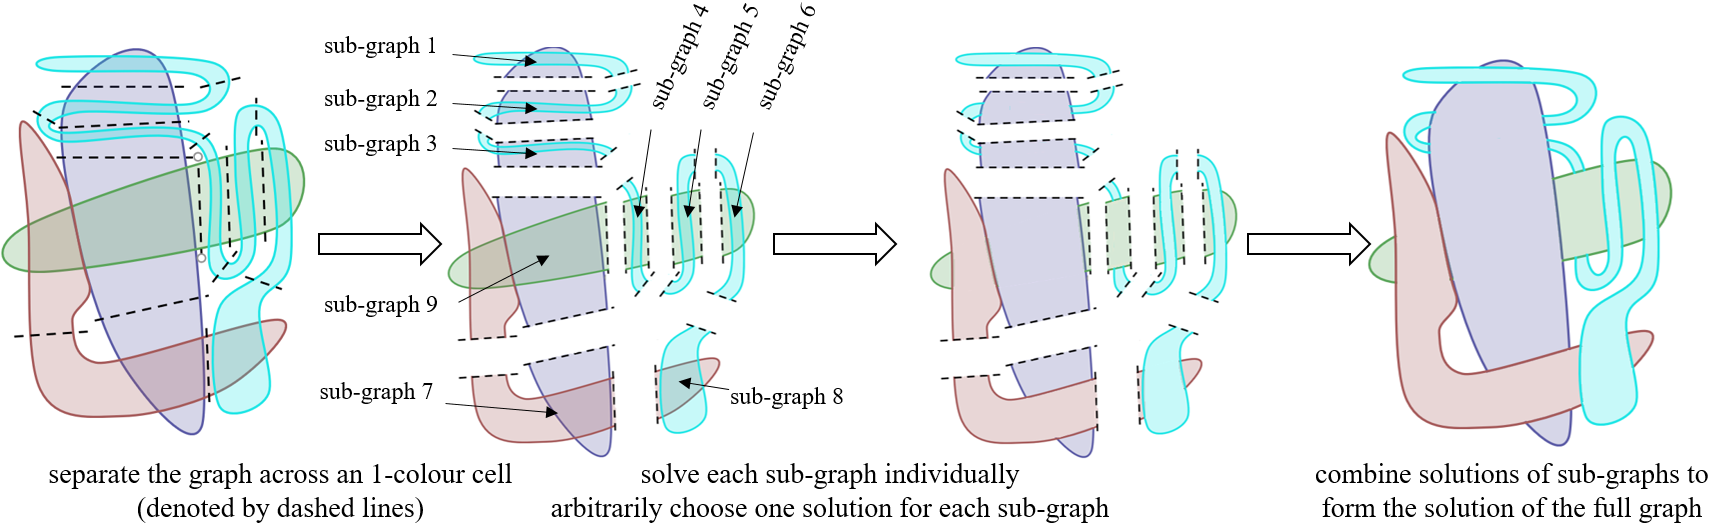
\includegraphics[width=\textwidth]{figures/two_overlapped_graph_2}
\caption{A maximally 2-overlapped graph to show the role of intersections. The full graph (left) is separated into $9$ sub-graphs through $1$-colour cells, shown with dashed cutting lines. Sub-graph $1$-$8$ has been shown to have two optimal solutions, while sub-graph $9$ gets a unique optimal solution after enumerative solving. Note that whatever solution gets chosen in each sub-graph, when two sub-graphs are combined, the two $1$-colour sub-cells separated by the dashed line re-join together, resulting in a reduction of one on the number of continuous regions. In total $4+(3\times 8)=28$ connected regions can be observed after solving the sub-graphs individually, combined with cost $-15$ (number of dashed lines). The nonrepetitive coverage problem of this graph ends up with $28-15=13$ connected regions, i.e., $12$ lift-offs. 
Note that no intersections in the full graph are avoided when solving all the sub-graphs. And different choices of the solution for each sub-graph will double the number of optimal solutions of the full graph: there will be $2^8=256$ optimal solutions to the graph.
}
%The number of continuous regions is $4+(3\times 8) = 28$  \textcolor{red}{??}, and $15$ dashed lines are created  \textcolor{red}{why? you say what you do, not why?}, so the number of continuous regions in the original graph is $28-15=13$, i.e., $12$ lift-offs are necessary to finish this coverage task. However, for all optimal cellular decompositions, each intersection has to be enumerated. The total number of optimal cellular decompositions will be $2^8 = 256$ \textcolor{red}{why?}, and no two of them are equivalent under continuous modification of cell boundaries \textcolor{red}{is this apparent in the figure? I can't see it}. 
\label{fig:two_overlapped_graph}
\end{figure*}


\begin{corollary}\label{coro:enum}
(Unavoidability of Enumeration) All intersections have to be enumerated in order to identify all optimal NCPP solutions. 
\end{corollary}

We prove this by showing two aspects:  
\begin{enumerate}
\item Collecting all solutions of a single intersection requires enumeration. 
\begin{proof}
It is proven by example that even a structurally simplistic intersection (a generic multi-entry intersection), needs  to undergo an enumerative solving mechanism. 
The intuitive dual-colour intersection shown in Fig.~\ref{fig:basic_shape}, with $4$ ``entries'', is extended to a more generic case with an arbitrary even number of entries, as the case depicted in in Fig.~\ref{fig:multi_entry}, with 8 entries. 
%After simplifying the case by merging consecutive adjacent cells which have the same set of possible colours, the intersection will have $n$ (an even number) entries. 
Let the intersection have $n$ % <Tong> what if its odd? why say this? does not look "extended to an arbitrary number of entries", looks very specific. Why would a case like Fig 5 but 7 entries need to be different in this discussion?
% <ty> If n is odd, then "b, g, ..., b" the final letter will be the same as the first one, i.e., 1-th and n-th entry will have the same colour and it turns back to the confusing T-junction case: we can combine the entry, transform 7-entry case to 6-entry case. Another reason for even n is from the solution n/2+1, if n is an odd number then n/2 is not an integer. I add an "even" to the above sentence, see whether it is ok. 
% <Tong> I understand, but I feel this needs to be more apparent in the explanation, otherwise it feels like we are just using simple cases but not tackling the complex ones, and one is left questioning whether the same principles and explanations apply to the more complex cases too! I changed slightly to try and accomodate for this, wthout going into a lot of detail that will make it harder to undestand (I feel)
entries, with consecutive adjacent cells having been assigned alternate colours, ``b(lue), g(reen), b, g, $\cdots$". 
It is observed that for each adjacent cell (say the $i$-th, labelled cyclicly), if it is connected to any other adjacent cell through the intersection, then another two entries, $(i-1)$ and $(i+1)$, cannot be connected. So the minimal number of connected regions for an $n$-entry intersection is $\frac{n}{2}+1$. % <Tong> so is this also the case for the even case? I can see the number will not be an integer, but will the formula will hold (rounded) if even? otherwise what we area saying about the minimal number of connected regions is ONLY for even num. of entries? we don' say that explictly, I read this as a generic statement, without constraints ... 
However, note that whilst the optimal number can be directly deduced, to get all optimal cellular decompositions the intersection still needs to be enumeratively solved. 
For the $i$-th entry, two scenarios must then be separately regarded, as illustrated in Fig.~\ref{fig:multi_entry}: % <Tong> these are the two cases we show in Fig 5, correct? if so, we can refer to it here too-> ...regarded, as ilustrated in Fig 5: 
% <ty> fixed
(a) keeping itself disconnected so that entries $(i-1)$ and $(i+1)$ can be connected (Fig.~\ref{fig:multi_entry}, top-right), % <Tong> on Fig 5 right, top <ty> fixed
or (b) connecting it to other entries (Fig.~\ref{fig:multi_entry}, bottom-right). %<Tong> , Fig 5 right, bottom.   <ty> fixed
Both of them go to optimal cellular decompositions.
% <Tong> I ended up adding he below then ... if it feels correct we leave
It is intuitive that more complex intersections can be devolved into simpler cases through connecting entries, thus transforming higher-entry cases into simpler cases as the example above, ultimately requiring solving through enumerative cellular decomposition regardless.
\end{proof}
\item Intersections are not removed by graph separation. 
\begin{proof}
This can be revealed in solving a simple graph, a maximally $2$-overlapped graph, 
illustrated by Fig.~\ref{fig:two_overlapped_graph}.  
The key step is to separate the graph into sub-graphs by dividing $1$-colour cells connecting intersections. 
Since the divided cell only has a unique coverable colour, we divide one cell into two unconnectable cells (they belong to different sub-graphs), so the number of continuous regions on the graph should be the sum of continuous regions in the sub-graphs, minus the number of dashed lines. 
Moreover, we can arbitrarily combine the optimal solutions of sub-graphs to form the optimal solution of the original graph. 
However, it should be noted that while the computational cost of combining solutions of sub-graphs has been reduced, no intersection was removed. 
Intersections must be solved within the sub-graphs, and all optimal solutions collected through a full combination of the different solutions with 
intersections. 
\end{proof}
\end{enumerate}


The examples employed to illustrate the various scenarios discussed thus far are relatively simplistic, and include graphs where intersections 
could be easily distinguished. However, for more generic graphs the necessity of solving by full enumeration is compounded by the 
inability to fully identify the intersections. 




\begin{lemma}
(Uncountability of Intersections) Given a graph, except for the most trivial cases (with either $0$ or $1$ intersection), the number of intersections in the graph is not countable. 
\end{lemma}
\begin{proof}
Fig.~\ref{fig:two_overlapped_graph} sub-graph $9$ illustrates the case where two parallel (non-overlapping but touching) colour regions exist which are simultaneously crossed by a third colour. In this case, the graph cannot be trivially separated since the multi-colour cells are adjacent, with no $1$-colour cell in between. 
A more detailed study of this case is provided in  Fig.~\ref{fig:add}. It can be easily observed how the graph has only one intersection, as after the intersection between red colour and green colour is resolved, the graph will have no further intersections. % <Tong> what about blue and green that is also two colours intersecting?
% <ty> Do you mean the right-top subfigure? the blue and green colour only form T-junction so there is no intersection. 
However, a combination of intersection-free graphs can generate an intersection-one graph, namely ``$0$" + ``$0$" = ``$1$" (Fig.~\ref{fig:add}(b)). % <Tong> I feel this is an abuse of notation perhaps as it is, 0+0 is not 1 ;-) Do you think it is worth it adding such notation if it does not impede the reading too much (and we don't have to change any figures or maths, e.g. I(0), or intersection-0 as you use in Corllary 9?
% <ty> I think it is not suitable either we use 0+0=1(it is not true) or use I(0)+ I(0) = I(1)( it is too heavy since we use it only once). I think may be ``0" + ``0" = ``1" looks better. 
Similarly, after the blue colour (with an apparent intersection with the green colour) is removed, % <Tong? why apparent? it is there % <ty> I drew a wrong figure. Now it should be correct. 
the remaining graph still has an intersection, namely ``$1$" - ``$1$" = ``$1$" (Fig.~\ref{fig:add}(c)). 
A more generalised set of cases can be encountered as shown in Fig.~\ref{fig:three_overlapped_graph}. It is apparent how the introduction of more and more colours leads to highly coupled intersections, where even identifying intersections becomes non-trivial. 
\end{proof}




\begin{corollary}
No algorithm that can solve a graph with explicit intersection-decreasing, such as transforming an intersection-$n$ graph to an intersection-$(n-1)$ partly-solved graph.
\end{corollary}

It can be thus concluded that any graph solvers (including all existing solvers, and the one to be proposed in this work) will face an enumerative scheme, where there is no guarantee of an explicitly decreasing number of intersections as a graph gets gradually solved. 
%And only when the graph is finally solved, and each of the final cells preserves a single colour, will the graph be known to be intersection-free. % <Tong> this is a bit strange as straight after we say we are going to create intersection-free graphs, which we do before solving, to make the solution complexity better. So a bit contradictory perhaps ...?
% <ty> I think commenting out this sentence may make things less confusing. 


\begin{figure}[t]
\centering
\subfigure[A graph with $1$ intersection, removed after solving (intersection cell allocated red colour). ]{
	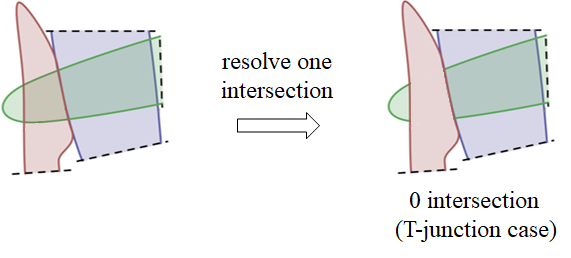
\includegraphics[width=0.4\textwidth]{figures/labelled_add_1}
% <Tong> complete this Fig., same as the others, the initial graph has one intersection, say so underneath, so all the same, as in c left 
}
\subfigure[Two intersection-free graphs form a graph with 1 intersection. ]{
	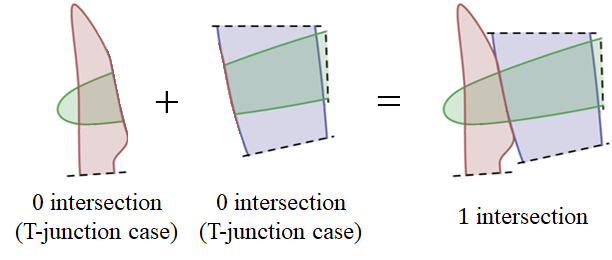
\includegraphics[width=0.4\textwidth]{figures/labelled_add_2}
}
\subfigure[After removing the blue colour together with its intersection with the green colour, the subgraph remaining % an intersection-one graph 
still has 1 intersection.]{
	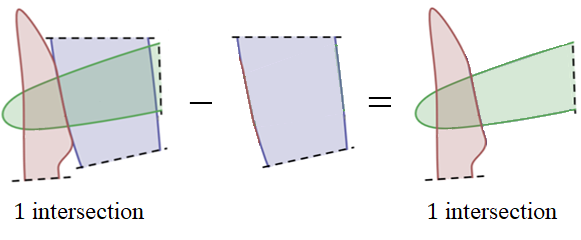
\includegraphics[width=0.4\textwidth]{figures/labelled_add_3}
% <Tong> is blue also an intersection? can we say so? (i.e. 1 intersection?) at the end of the day we say 1 - 1, meaning a graph with 1 intersection - a graph with 1 intersecton, correct?
}
\caption{Examples of intersection countability complexity as graphs gets resolved, depicting the interesting scenarios where (b) intersections are created from 0 intersection subgraphs (``$0$" + ``$0$" = ``$1$"), and (c) the same number of intersections remains even after removal of one of them (``$1$" - ``$1$" = ``$1$").% in the number of intersections between graph and sub-graphs. 
} % <Tong> add figure letters to the cases in the caption 
% <ty> added 
% <Tong> not the case, I meant refering to the subfibure letters in the caption. I added.
\label{fig:add}
\end{figure}


\subsection{Intersection-Free Graphs}
It has been discussed how disregarding the position of intersections and how to solve them leads to exhaustive implicit enumeration when 
all edges and cells are enumerated~\cite{Yang2020Cellular}. 
On the other hand, exploiting the interesting complex scenarios that analysing the topology between different colours offer will attenuate 
this problem. In this regard, the concept of intersection-free graphs plays a crucial role.  

\begin{definition}
(Intersection-free Graph) An intersection-free graph is a graph where no intersection can be constructed within it. 
\end{definition}
% <Tong> should this not be a definition in itself? the layout as it it now is not very nice, with a funny identation ... % <ty> fixed
Two types of cells can be distinguished in a graph: 
\begin{definition}
(Boundary Cell, Internal Cell) \textit{Boundary cells} are the cells which have edges forming the boundary of the graph. 
The remaining cells are \textit{internal cells} which have no edge exposed to the graph boundary. 
\end{definition}
See Fig.~\ref{fig:characteristic_string} for illustration of an intersection-free graph with $6$ boundary cells and $2$ internal cells. 
It is apparent that all internal cells are shown to have less than $4$ cells, or else an intersection could be constructed within. 


\begin{definition}
(Characteristic String) Given a graph, let there be $n$ (ordered) boundary edges, then the characteristic string of the graph is a word of length $n$, where the $i$-th letter in the word represents the colour of the boundary cell containing the $i$-th boundary edge. 
\end{definition}

For the example in Fig.~\ref{fig:characteristic_string}, the partly painted graph has characteristic string ``[b, b, r, r, r, g]". 
A crucial property of intersection-free graphs is presented as the following theorem:
\begin{theorem}\label{thm:string}
The solution of the graph, i.e., the assigned colour of all cells in the graph, can be uniquely characterised by the colour of the boundary cells. 
\end{theorem}



\begin{figure}[t]
\centering
\subfigure[]{
	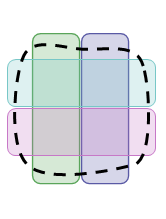
\includegraphics[height=0.07\textwidth]{figures/2_2_intersection}
}
\subfigure[]{
	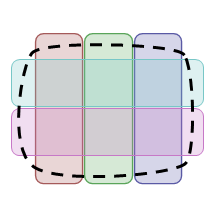
\includegraphics[height=0.07\textwidth]{figures/2_3_intersection}
}
\subfigure[]{
	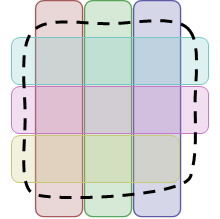
\includegraphics[height=0.07\textwidth]{figures/3_3_intersection}
}
\subfigure[]{
	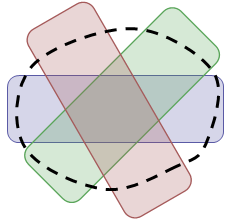
\includegraphics[height=0.07\textwidth]{figures/3_intersection}
}
\subfigure[]{
	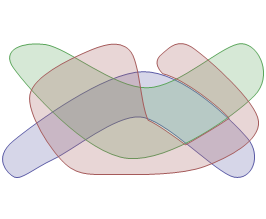
\includegraphics[height=0.07\textwidth]{figures/3_intersection_2}
}
\caption{Graphs with ever increasing complex intersection scenarios. 
%The dashed circle marks the part of the graph containing intersections. 
Intersections are contained with the encircled dashed line, whilst intersection entries lay in the outside. 
Intersection in these examples are formed by: (a) $2\&2$ parallel colours, (b) $2\&3$ parallel colours, (c) $3\&3$ parallel colours, 
%a further special case of $3\&3$ parallel colours (where whether the orange colour intersects with the blue colour is closely related to the optimal solutions. Now they only form a T-junction), 
(d) a normal $3$-overlapped intersections, and (e) a complex $3$-overlapped graph where delineation of the intersecting section in the graph 
is not apparent given the many intersections and paralleled colours within.}
\label{fig:three_overlapped_graph}
\end{figure}


\begin{figure*}[t]
\centering
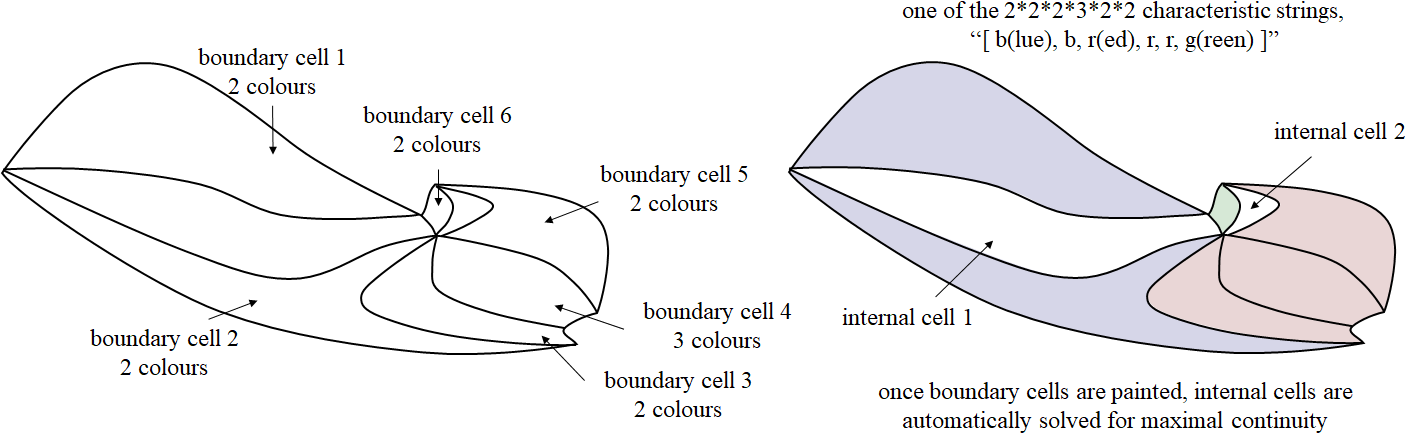
\includegraphics[width=0.9\textwidth]{figures/characteristic_string_2}
\caption{An intersection-free graph. The internal cell $1$ will choose blue $>$ green $>$ other colours. The internal cell $2$ will choose green $=$ red $>$ other colours.}\label{fig:characteristic_string}
\end{figure*}


\begin{proof}
Let the colour of all boundary cells be determined. On picking up two boundary cells with the same colour one must be able to judge their connectivity through this graph. Should connectivity be undetermined, one may find another pair of boundary cells whose connection may prevent these two cells from being connected. However, this represents an intersection, which contradicts the intersection-free assumption of the graph. 

%The colour of the (ordered) boundary cells can be recorded in a string with length equalling the number of boundary edges of the graph, referred to as 
%the \textit{characteristic string} of the graph. 
After assigning a colour to each boundary cell, all internal cells will be assigned the colour which maximises the connectivity to their adjacent cells. 
After all cells have had their colour allocated, all the internal edges can be  automatically solved. 
It can thus be said that each characteristic string uniquely corresponds to a solution of the intersection-free graph, 
and the number of characteristic strings can then be likened to the full quantification of the number of solutions in the graph. 
\end{proof}
\begin{figure}[t]
\centering
\subfigure[]{
	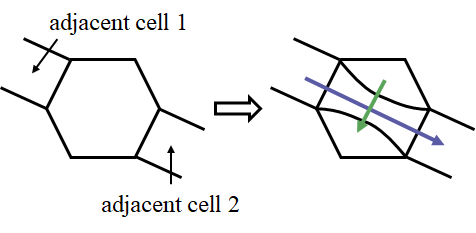
\includegraphics[width=0.22\textwidth]{figures/constraint_violation_a_2}
}
\subfigure[]{
	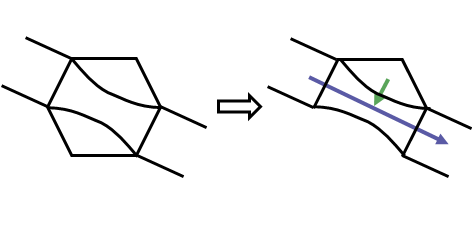
\includegraphics[width=0.22\textwidth]{figures/constraint_violation_b_2}
}
\caption{(a) Illustration of constraint violation due to cell sub-divisions in sub-graphs. One sub-cell will have four adjacent cells. (b) If a cell is scheduled to be divided, it should first be divided and then followed by constructing the intersection-free sub-graphs.}
\label{fig:constraint_violation}
\end{figure}

\section{Graph Separation}
\label{section_graph_separation}
An efficient strategy to separate a graph into intersection-free sub-graphs is described in this section. 
The reader is referred to the algorithm pseudocode given in \textbf{Algorithm}~\ref{alg:1}.
Since non-adjacency of internal cells in sub-graphs will be enforced, and cell sub-divisions after sub-graphs have already been constructed, 
this constraint may be violated (see Fig.~\ref{fig:constraint_violation} for an illustration of this scenario).
So let at this point all $n(\geq 4)$-edge cells be assumed properly divided before applying the algorithm. As such, 
all cells contained in the sub-graphs can only be seen as a whole, and be filled with the same colour. 

An apparent result for graph separation is that the graph should not be separated across edges, or else the constraints of the original cell vanishes, and non-optimal solutions may appear. 
See an illustration of this scenario in Fig~\ref{fig:separation_at_edges}. 
Another result is that the optimality of part of the graph has no relation to the global optimal solution of the whole graph. 
This is proved by the example illustrated in Fig~\ref{fig:local_combined}. 

\begin{figure}[t]
\centering
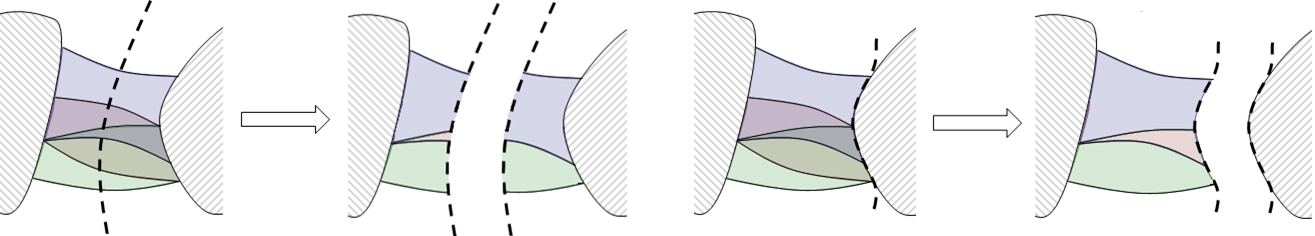
\includegraphics[width=0.48\textwidth]{figures/separation_at_edges_2}
\caption{If a graph is separated through division of multi-colour cells, the constraint of the cell vanishes, then in the sub-graphs there may exist solutions that after being combined is non-optimal, such as the case given in left. If the graph is separated along edges, we will not incur such problem. }\label{fig:separation_at_edges}
\end{figure}


%\subsection{Relation between Optimality of Graph and Its Sub-Graphs}
%Before we go into relations between graph and sub-graphs, we have to claim a basic criteria for separating a graph into sub-graphs. 
%Different from separating the graph through an $1$-colour cell, where the solutions of sub-graphs can be arbitrarily combined, if we separate the graph through multi-colour cells, as illustrated in Fig.~\ref{fig:separation_at_edges}, the constraints of the original cell vanishes, then proven non-optimal solutions may appear. In contrast, separating the graph through existing edges has the same effort, which is desired. 
%So in sequel our graph separation process should  follow existing edges in the graph, which makes Fig.~\ref{fig:non_optimal_subgraph} and Fig.~\ref{fig:local_in_other_graph} reasonable. 

%It is also observed that if the edge has multi-colour adjacent cells, then the combination of different solutions of sub-graphs will have non-trivial cost variation (not $-1$ as used in Fig.~\ref{fig:two_overlapped_graph}). 

\begin{figure}[t]
\centering
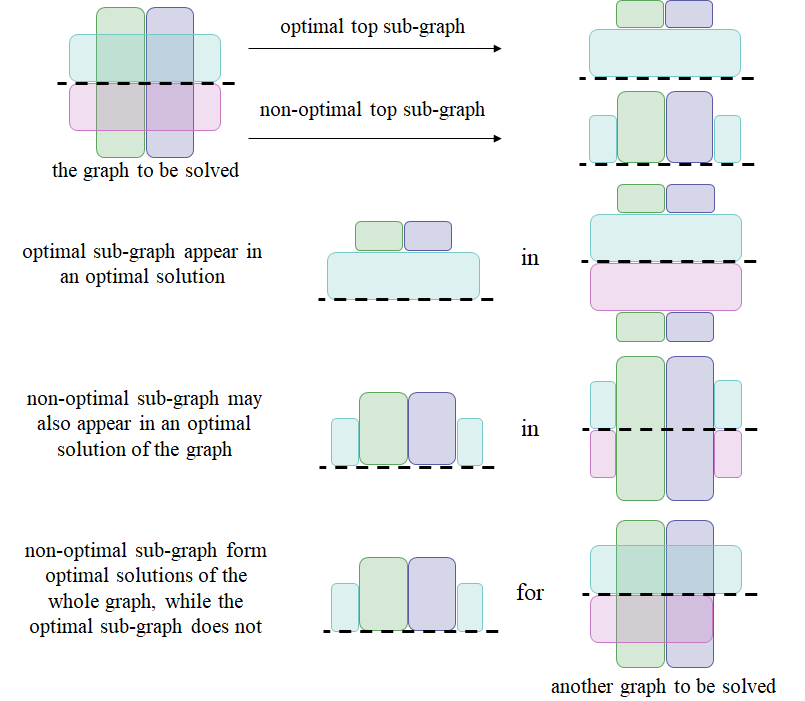
\includegraphics[width=0.48\textwidth]{figures/local_combined}
\caption{Separating the graph through the dashed line, we show the optimal solution and a non-optimal solution of the sub-graph. It is noticeable that both of them form optimal solutions of the original graph. An in the bottom case, as a sub-graph of another graph, the non-optimal sub-graph can form optimal solutions while the optimal sub-graph cannot do so. }\label{fig:local_combined}
\end{figure}

%Then, we claim that there is no guarantee about the global optimality of combining optimal solutions of sub-graphs. In other words, when a graph is separated into sub-graphs, we have to collect all solutions of each sub-graph. (It is not a bad thing if all solutions of sub-graphs can be enumerated, since in this case solving sub-graphs is unnecessary. )
%This is proved by two examples illustrated in Fig.~\ref{fig:non_optimal_subgraph} and Fig.\ref{fig:local_in_other_graph}. In \ref{fig:non_optimal_subgraph} both optimal and non-optimal solution of the sub-graph will form an optimal solution of the original graph. And in Fig.\ref{fig:local_in_other_graph} it is shown that non-optimal sub-graph is included in optimal solution of the original graph while the optimal sub-graph is not. 
%See Fig.\ref{fig:non_optimal_subgraph}, where the graph to be solved is an intersection between three parallel colours and another three parallel colours. The optimal solution is obviously either connecting all horizontal colours or connecting all vertical colours. 
%We can see from this case that optimality of the sub-graph is not equivalent to the optimality of the whole graph. So if a graph is separated into sub-graphs, we should store all solutions of sub-graphs but not only optimal solutions. 
%Another problem is that the optimality of a solution of the sub-graph hugely depends on other sub-graphs. A case is given in Fig.\ref{fig:local_in_other_graph}. 
%So we can only judge the optimality after we pick one solution from each sub-graph and combine them to form a solution of the whole graph. 
%In other words, in the absense of arbitrary combination of the solutions of sub-graphs, the algorithmic complexity of the graph is the multiplication but not the sum of the complexity of solving each sub-graph. 


\begin{algorithm}[t]
    \caption{Improved Solver}\label{alg:1}
    \begin{algorithmic}[1]
        \Require The initial graph $G = (\{C_i\}_{i = 1}^M, \{E_j\}_{j = 1}^N)$  
        \Ensure All solved graphs $\{result\}$  
\For{all $E_1$ ways of divisions of cell $1$} 
\If{non-optimality is detected}
\State \textbf{continue}
\EndIf
\State $\ddots$
	\For{all $E_M$ ways of divisions of cell $M$}
	\If{non-optimality is detected}
	\State \textbf{continue}
	\EndIf
	\State // Graph Separation into Strips (Section~\ref{section_graph_separation})
		\While{the graph is not intersection-free}\label{alg:separation_start}
		\State Choose a cell to be in the new strip
		\State Attach new cells satisfying constraints
		\State separate the strip from the graph
		\EndWhile\label{alg:separation_end}
		\State // Let there be $n$ strips generated
		\State // Enumerate solutions by characteristic strings 
		\State // (\textbf{Theorem}~\ref{thm:string})
		\For{all characteristic strings of strip $1$}
		\State $\ddots$
		\For{all characteristic strings of strip $n$}
		\State Combine strips to form a solution $S$\label{alg:combining_start}
		\If{it is better than $\{result\}$}
		\State $\{result\} = \varnothing$
		\State push $S$ into $\{result\}$
		\Else
		\If{it is currently optimal}
			\State push $S$ into $\{result\}$
		\EndIf
		\EndIf\label{alg:combining_end}
		\EndFor
		\State $\udots$
		\EndFor

	\EndFor
\State $\udots$
\EndFor% cell 1 sub-division
    \end{algorithmic}  
\end{algorithm}


\begin{figure*}[t]
\centering
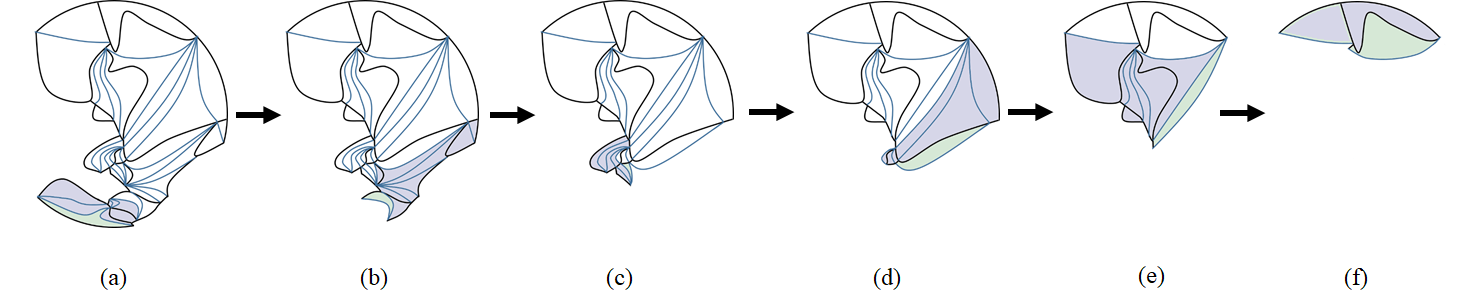
\includegraphics[width=0.96\textwidth]{figures/steps_2}
\caption{Step-by-step illustration of the separation of the graph shown in Fig.~\ref{fig:complicated_graph} into intersection-free strips. The light green cell is the first one selected to form a new strip, and all light purple cells are then inserted into the same strip. The graph ends up with $6$ separated strips.}
% <Tong> pls add a bit more in the caption to better describe what it is, each region of coloured cells is a Strip, ending up with 6 ... just a bit more descriptive. NOT major wording!! MINOR, just detailing 
% <ty> added
\label{fig:steps}
\end{figure*}

\begin{figure*}[t]
\centering
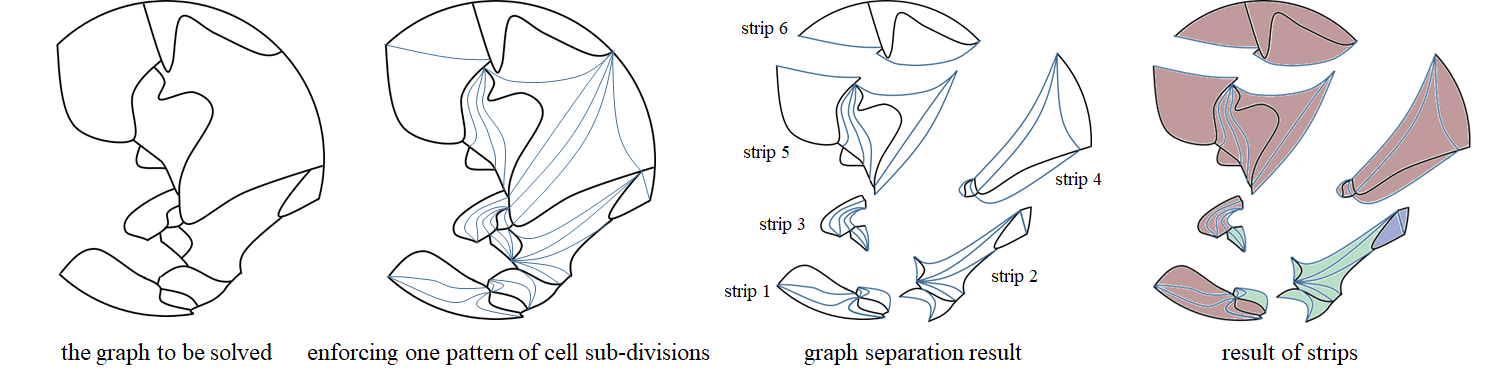
\includegraphics[width =0.96\textwidth]{figures/graph_separation_3}
\caption{Illustration of how an unsolved graph is separated into strips. }\label{fig:complicated_graph}
\end{figure*}


\subsection{Definition of Strips}
\begin{definition}\label{def:strip}
(Strip) A strip is a graph designed such that 
\begin{enumerate}
\item Each cell has at most $3$ adjacent cells, and
\item Internal cells are non-adjacent, 
\end{enumerate}
\end{definition}

%\begin{proposition}
%\label{proposition:strips}
%In a graph designed such that 
%\begin{enumerate}
%\item Each cell has at most $3$ adjacent cells, and
%\item Internal cells are non-adjacent, 
%\end{enumerate}
%then the graph is an intersection-free graph. 
%\end{proposition}
\begin{proposition}\label{proposition:strips}
Strips are intersection-free graphs. 
\end{proposition}
\begin{proof}
It is observed that when a section of a graph contains an intersection, there must exist at least $4$ entries. 
Moreover, each entry may not occupy a single edge.  
These motivate us to consider its opposite: if condition 1) in \textbf{Definition}~\ref{def:strip} is satisfied, then there can not possibly be an intersection. 
In noting that two internal $3$-edge cells may form a $4$-edge cell which breaks this criterion, condition 2) is required. 
\end{proof}



%With all internal cells being isolated, a graph satisfying the above two constraints is referred to as a \textit{strip}. 


\subsection{Graph Separation into Strips}
At this point in the start of the separation process it can be safely assumed that all multi-edge cells have been divided. 
Please refer to Fig.~\ref{fig:steps} for a visualisation of the separation process with an example.

 One boundary cell is first selected and regarded as an element of strip $1$, shown in light green in Fig.~\ref{fig:steps}(a).
Each cell adjacent to the strip is checked to validate whether accommodating the cell into the strip will violate the strip constraints (\textbf{Definition}~\ref{def:strip}). Otherwise it is inserted. 
When no further cells can be inserted, the construction of strip $1$ is deemed finished. 
In this example, as shown in Fig.~\ref{fig:steps}(a), adjacent cells are iteratively inserted to strip $1$ which are shown in blue. If one more cell is inserted, then the boundary cell $5$ (illustrated in detail in Fig.~\ref{fig:characteristic_string}) will become an internal cell which is adjacent to the internal cell $2$, so the construction of strip $1$ terminates.  

% <Tong> pls add a bit more references to Fig 13 (b, c) in the txt below. e.g. Strip 2 is Fig 13b
% <ty> added
To construct strip $2$ (Fig.~\ref{fig:steps}(b)), a cell (shown in light green) adjacent to strip $1$ is selected, then its adjacent cells are checked one-by-one to see whether they can be inserted respecting the conditions in \textbf{Definition}~\ref{def:strip}. 
After that, another cell in the left-out graph is chosen into strip $3$ (Fig.~\ref{fig:steps}(c)), and other cells are again checked and attempted to be inserted into strip $3$, and so on. 
By iteratively considering adding the adjacent cells to the previous strip into the current strip and adding more cells satisfying the two constraints, 
the whole graph can be finally separated into strips, as shown in Fig.~\ref{fig:complicated_graph} where the graph is separated into $6$ strips. (The process corresponds to line \ref{alg:separation_start} $\sim$ line \ref{alg:separation_end} in \textbf{Algorithm} \ref{alg:1}.) 

% <Tong> we seem to use indistinctively the term subgraph and intersection-free strips in this section, and pictures used. I feel adds some mild, if unnecesary confussion. I've modified some bits, but have a closer read see whether you can see spots where that can be avoided. For instance the caption of fig 13 and 14? 
% Pls note MINOR modifications, simply add/remove spefici words is what I'm after
% <ty> Not totally sure what do you want me to modify. In this version I would like to make "sub-graph" to be a general description of the result of the graph separation process, while the "strip" to be the intersection-free structure that we construct. In particularly, I think the current Def 14 and Prop 15 is the suitable order for defining strips. Please see whether it helps to make anything clearer. 



\subsection{Solving Strips}
After the graph has been separated, all the solutions for each strip are enumerated via iterating through all the possible characteristic strings. 
Note that there is no extra memory cost for this step - all strip solutions are indexed by the characteristic strings, so they can be randomly accessed 
to be able to pick up any solution of one strip to combine with other strips, resulting in a given solution to the original graph. 

\subsection{Full Graph Solution}
Picking up one solution from each sub-graph, they are combined to form a solution of the original graph. 
The edges identified during the graph separation process are automatically solved by comparing the colour of its two adjacent cells. 
A cost is calculated whose physical meaning is the number of connected regions in the painted part of the (combined) sub-graphs~\cite{Yang2020Cellular}. 
Once the original graph is re-constructed, the number of connected regions in the solution is fully known. Its optimality can be trivially judged against all possible combinations of sub-graph solutions to reach a set with all the optimal solutions. (line \ref{alg:combining_start} $\sim$ line \ref{alg:combining_end} in \textbf{Algorithm} \ref{alg:1})

\section{Complexity}
\label{section_complexity}
The advancement that the proposed mechanism brings about in solving the NCCP problem is reflected in an exponential improvement in algorithmic complexity over existing approaches.

As mentioned earlier, cell sub-divisions were undertaken before graph separation to avoid the possible  constraint violation caused by cell sub-divisions in strips. So the algorithm complexity must also be calculated based on this (i.e. no $\prod E_i$ is multiplied for that segment of the procedure).

\begin{theorem}
Given a topological graph to be solved, it is assumed that it has been first cell sub-divided before running the enumerative solvers. Let there be $M$ topological cells and $N$ internal edges in the graph. The number of edges for the $i$-th cell is $\alpha_i$, and denote the number of available colours to fill cell $i$ as $K_i$. Then, the proposed graph separation-based algorithm encompasses the following number of steps for enumerative solving the graph:
\begin{equation}
\prod\limits_{j = 1}^M K_j^{\max\{\alpha_j-2, 1\}}
\end{equation}
Compared to the complexity of the full enumeration solution~\cite{Yang2020Cellular}
\begin{equation}
\prod\limits_{j = 1}^M K_j^{\max\{\alpha_j-2, 1\}}\cdot 2^N
\end{equation}
the proposed graphing scheme represents an exponential improvement in 
the order of $2^N$. 
\end{theorem}


\begin{proof}
%The proposed algorithm has been shown to consist of a number of steps: (1) separating a graph into subgraphs, (2) separating each subgraph into strips, solving each strip individually, and constructing all optimal solutions by combining the individual strip solutions. Finally (3) all individual subgraph solutions can be combined to form the solutions to the original graph. 
The proposed algorithm has been shown to consist on a number of steps, namely: 
\begin{enumerate}
\item Separating a graph into strips 
\item Solving each strip individually. 
\item Constructing all optimal solutions of the original graph by combining the individual strip solutions. 
\end{enumerate}

\noindent
The overall complexity can thus be calculated individually for each step. 

1) Separating the graph only requires checking on each cell once, and we only need one valid graph separation, so the complexity of this part is denoted by $\Phi = O(M)$. 

2) The complexity of a single strip can be derived as follows: Let there be $r_i$ boundary cells and $s_i$ internal cells in the strip $i$, 
indexed as $( i_1, \cdots, i_{r_i}, i_{r_i+1}, \cdots, i_{r_i+s_i})$, 
and having $(\alpha_{i_1}, \cdots, \alpha_{i_{r_i}}, \alpha_{i_{r_i+1}}, \cdots, \alpha_{i_{r_i+s_i}})$ edges. 
The number of available colours for each cell can be  written as $(K_{i_1}, \cdots, K_{i_{r_i}}, K_{i_{r_i+1}}, \cdots, K_{i_{r_i+s_i}})$. 
Note that the list of cells form a chain, so that other than the start and end cells, each cell will have two internal edges, one shared with its precedent cell and the 
other shared with its successor. As a 2D topological structure, a cell $j$ in the strip will have at least two internal edges, and at most $(\alpha_{i_j}-2)$ edges are exposed to the boundary of the strip. 
Hence, the complexity $\Psi_i$  of solving strip $i$ will be the multiplication of the algorithmic complexity of all boundary cells 
\begin{equation}
\Psi_i = \prod\limits_{j = 1}^{r_i} K_{i_j}^{\max\{\alpha_{i_j}-2, 1\}}
\end{equation}
where $\max\{\alpha_{i_j}-2, 1\}$ represents the case that multiple edges of the same cell may appear in the strip boundary. 
Since the enumeration of the solutions for different strips is fully independent, the combined complexity is just summed up but not muliplied. 
Considering the notation $M = \sum (r_i+s_i)$, the overall complexity of finding the solutions for a sub-graph is given by
\begin{equation}
\begin{aligned}
\Psi = \sum \Psi_i = & \sum\limits_{i} \left(\prod\limits_{j = 1}^{r_i} K_{i_j}^{\max\{\alpha_{i_j}-2, 1\}}\right)\\
\ll & \sum\limits_{i} \left(\prod\limits_{j = 1}^{r_i+s_i} K_{i_j}^{\max\{\alpha_{i_j}-2, 1\}}\right)\\
\ll&\prod\limits_{i}\left(\prod\limits_{j = 1}^{r_i+s_i} K_{i_j}^{\max\{\alpha_{i_j}-2, 1\}}\right)\\
=&\prod\limits_{j = 1}^M K_j^{\max\{\alpha_j -2, 1\}}
\end{aligned}
\end{equation}

3) For the final step of the algorithm, the complexity is the multiplication of the algorithmic complexity of all sub-graphs 
\begin{equation}
\begin{aligned}
\Xi = \prod \Psi_i = & \prod\limits_i \left(\prod\limits_{j = 1}^{r_i} K_{i_j}^{\max\{\alpha_{i_j}-2, 1\}}\right)\\
\ll&  \prod\limits_i \left(\prod\limits_{j = 1}^{r_i+s_i} K_{i_j}^{\max\{\alpha_{i_j}-2, 1\}}\right)\\
\ll& \prod\limits_{j = 1}^M K_j^{\max\{\alpha_j-2, 1\}}
\end{aligned}
\end{equation}
The overall complexity of the proposed algorithm is the sum of $\Phi$, $\Psi$ and $\Xi$, 
\begin{equation}
\Gamma =\Phi+\Psi+\Xi \ll  \prod\limits_{j = 1}^M K_j^{\max\{\alpha_j-2, 1\}}
\end{equation}
\end{proof}

\begin{comment}
Compared to the complexity of the full enumeration solution~\cite{Yang2020Cellular}
\begin{equation}
\prod\limits_{j = 1}^M K_j^{\max\{\alpha_j-2, 1\}}\cdot 2^N
\end{equation}

It can be observed how the proposed graphing scheme represents an exponential improvement in 
the order of $2^N$, with $N$ being the number of topological edges in the graph. 
\end{comment}

%\begin{figure*}[t]
%\centering
%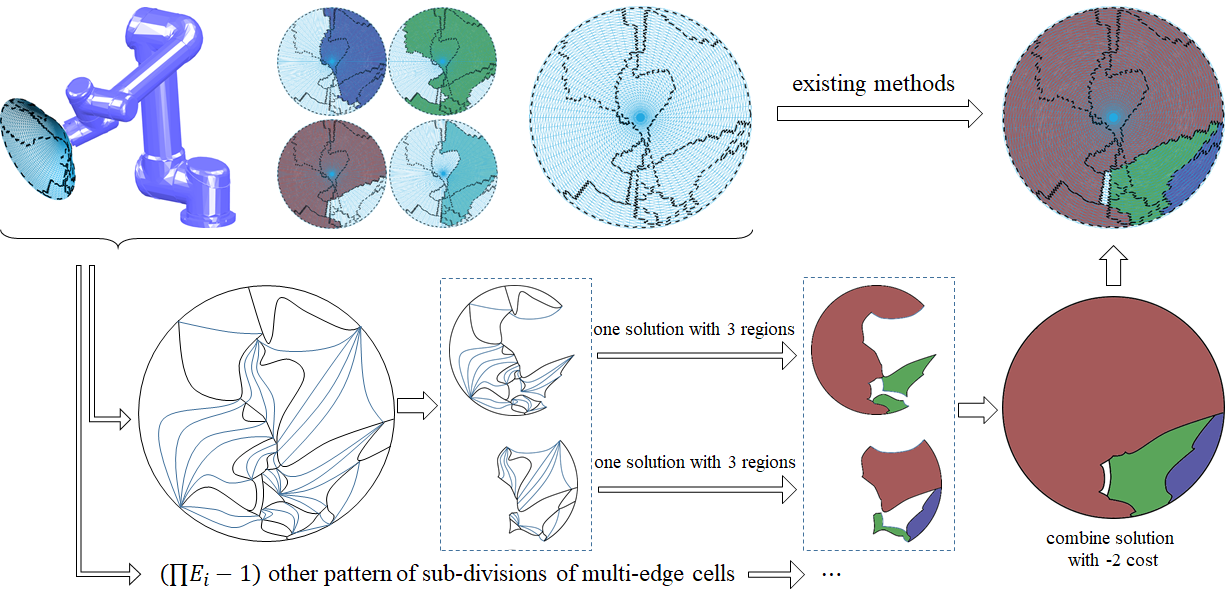
\includegraphics[width = 0.96\textwidth]{figures/hat_exp/fig_hat}
%\caption{\textcolor{blue}{What if I directly use the sub-graph in this experiment to be the demo figures of the above algorithm section? }}\label{fig:hat}
%\end{figure*}

\begin{figure}[t]
\centering
\subfigure[]{
	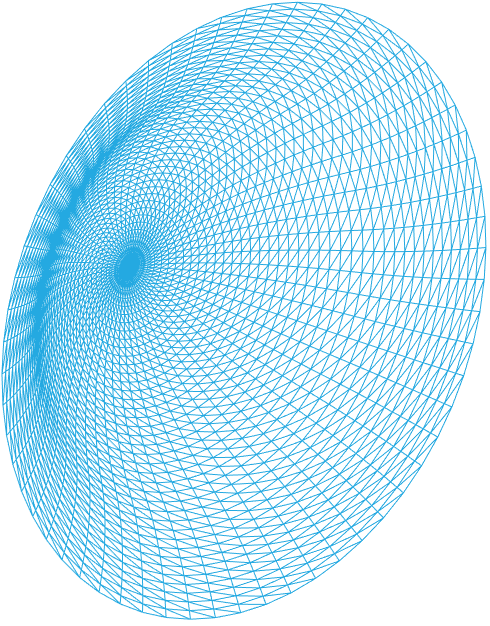
\includegraphics[width=0.15\textwidth]{figures/hat_exp/mesh}
}
\subfigure[]{
	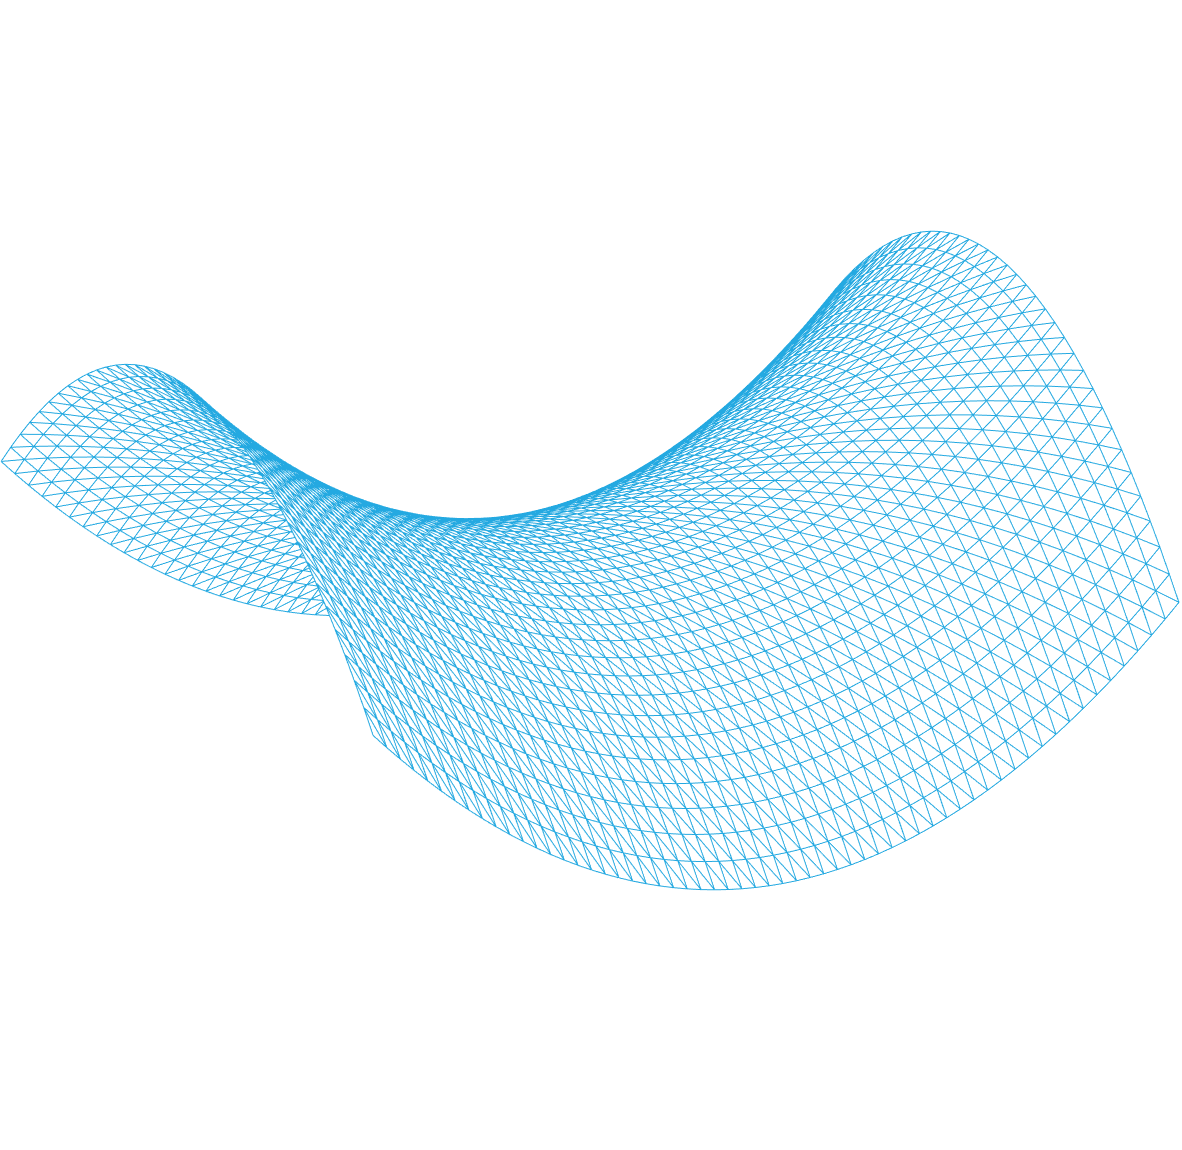
\includegraphics[width=0.15\textwidth]{figures/saddle_exp/mesh}
}
\caption{The objects used to experimentally illustrate the results, Section~\ref{section_results}.}
\label{fig:object}
\end{figure}

\begin{figure*}[t]
\centering
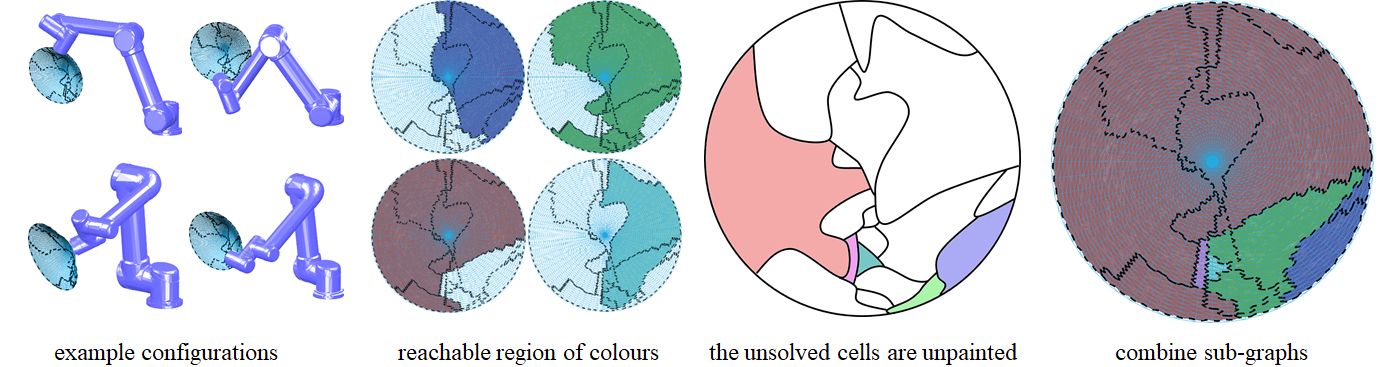
\includegraphics[width=0.96\textwidth]{figures/hat_exp/fig_hat_2}
\caption{The coverage task of a hat-shape object. The reachable area of different colours and one of their corresponding configurations are depicted. After painting all $1$-colour cells, the unsolved graph is %exactly the same one as we have discussed in Section \ref{section_graph_separation}. }
separated and solved as decribed in Section~\ref{section_graph_separation}, with the step-by-step process illustrated in Fig.~\ref{fig:steps} } % <Tong> I changed this, pls check ok
\label{fig:hat}
\end{figure*}
\begin{figure*}[t]
\centering
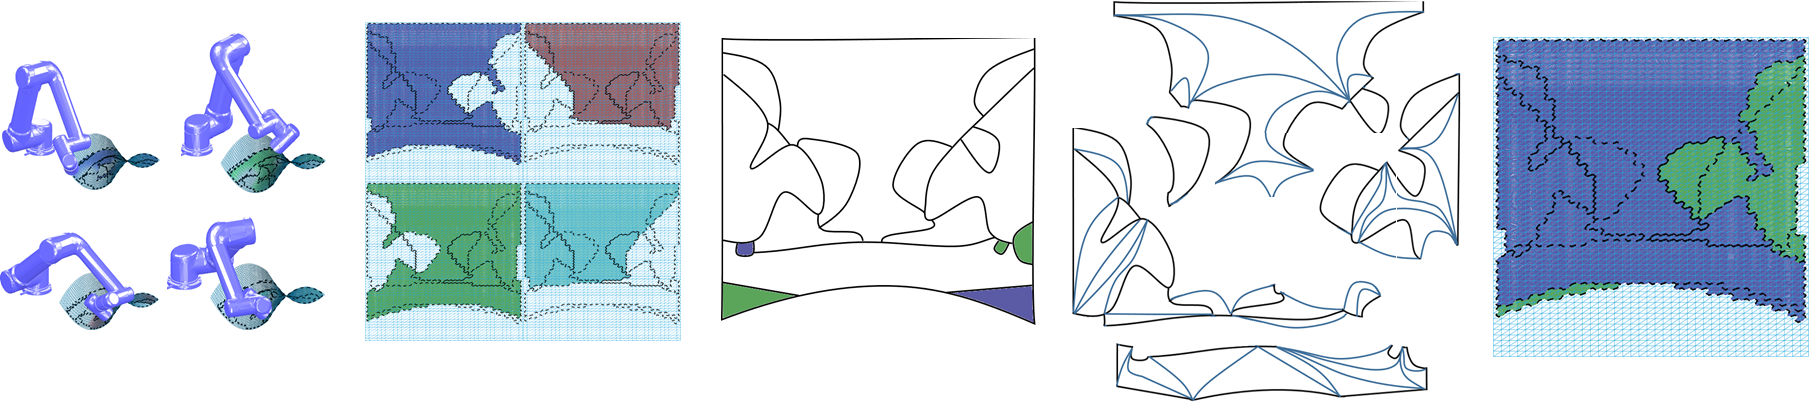
\includegraphics[width=0.96\textwidth]{figures/saddle_exp/comb}
\caption{The coverage task of a saddle surface. The reachable area of different colour and one of their corresponding configurations are depicted. After painting all $1$-colour cells, the unsolved grpah is separated into $5$ sub-graphs. Finally, all optimal solutions can be collected with 2 end-effector lift-offs.}
\label{fig:saddle}
\end{figure*}

\section{Experimental Results}\label{section_experiment}
\label{section_results}

The proposed solution is tested experimentally by simulating the NCPP with a non-redundant manipulator (6 DoF Universal Robot UR5) on two arbitrarily shaped objects, one a hat-like concave semi-sphere (only one side is considered), and a saddle surface (only one side being considered also), as shown in Fig.~\ref{fig:object}.

\subsection{Optimal NCPP on a Hat-shape Object}
% <ty> Suddenly I notice that the demo figure is not illustrative. Will change
An illustration of the solving process for the hat-shape object is depicted in Fig.~\ref{fig:hat}. 
Four continuous sets of manipulator configurations are represented in blue, red, green and cyan colour separately. $1$-colour cells have been directly drawn to the graph. 
%Using existing algorithms~\cite{Yang2020Cellular}, the initial topological graph is directly enumerated. We need to iteratively decide whether keep/remove each topological edges, and choose colour for each (sub-)cells, leading to complexity as (\ref{equ:tmech}). One of the graph after cell sub-divisions is shown in Fig.~\ref{fig:hat}.  
The cell sub-divisions correspond to the description provided earlier in Fig.~\ref{fig:complicated_graph}.
For the algorithmic complexity there are $43$ cells. The possible colours of each cell are known. As for edges, there are $44$ unsolved edges (drawn in black) and $30$ manually created edges - enforced to be kept (drawn in blue). Plus $9$ edges which are connected to unreachable area (a fifth colour), which need not solving. Using the naive enumeration proposed in the literature, %~\cite{Yang2020Cellular} - we've repeated this too many times I feel
$35$ edges and all colours of all cells are enumerated, resulting in an algorithmic complexity described by 
\begin{equation}
{\color{red}2^{35}\times}
\begin{aligned}
&\overbrace{2\times2\times3\times2\times2\times2\times{\color{red}2\times2\times}}^{\textbf{all cells in sub-graph 1, shown in Fig.~\ref{fig:characteristic_string}}}\\
&2\times3\times3\times2\times2\times3\times2\times3\times2\times{\color{red}3\times}\\
&2\times2\times2\times2\times2\times2\times{\color{red}2\times}\\
&2\times3\times3\times4\times4\times{\color{red}3\times4\times}\\
&3\times3\times2\times3\times3\times4\times4\times{\color{red}3\times}\\
&3\times4\times3
\end{aligned}
\approx 1.2705\times10^{28}
\end{equation}
Please note there is a minor abuse of notation in the arrangement of the numbers above simply so that they can be easier to compared with the optimal solution below. 
%\begin{equation}
%2^{35}\cdot \underbrace{2\times 2\times \cdots \times 3}_{43 \mbox{ terms, number of colours}} \approx 1.2705*10^{28}
%\end{equation}

Using the proposed algorithm, the length of the boundary for each sub-graph is $6, 11, 9, 6, 10, 5$ respectively. The reader is referred to the sub-graph $1$ example
employed to discuss the process in detail in Sections~\ref{section_intersection} and~\ref{section_graph_separation}. Detail results for the others cases are ommited for lack of space, 
but follow the same process. 
The number of colours for the boundary cells in each sub-graph is included in the multiplicative factor, so the algorithm complexity derives in the multiplication of 
the complexity of all sub-graphs, given by 
\begin{equation}
\begin{aligned}
&\overbrace{2\times2\times3\times2\times2\times2\times}^{\textbf{internal cells shown in Fig.~\ref{fig:characteristic_string}}}\\
&2\times3\times3\times2\times2\times3\times2\times3\times2\times\\
&2\times2\times2\times2\times2\times2\times\\
&2\times3\times3\times4\times4\times\\
&3\times3\times2\times3\times3\times4\times4\times\\
&3\times4\times3
\end{aligned} \approx 4.2797\times10^{14}
\end{equation}

\subsection{Optimal NCPP on a Saddle-shape Object}
Another example is provided with the analysis of the outer shell of a saddle-shape object. In this case the surface normal varies greatly as the end-effector moves 
along the surface, representing a challeging manipulator planning problem in adopting poses that would benefit the continuous coverage this paper is interested in. 
The algorithmic complexity given cell sub-divisions is shown in Fig.~\ref{fig:saddle}. For the  naive enumeration case, the overall complexity is given by 
%\begin{equation}
\begin{flalign}
&{\color{red}2^{47}*}~
\begin{aligned}
&2\times2\times2\times2\times2\times2\times2\times2\times2\times{\color{red}2\times}\\
&3\times2\times2\times2\times2\times2\times2\times \\
&~~~~3\times4\times4\times3\times2\times2\times2\times3\times{\color{red}3\times}\\
&3\times2\times2\times2\times2\times3\times3\times2\times{\color{red}2\times}\\
&4\times4\times4\times4\times4\times4\times3\times4\times{\color{red}4\times}\\
&3
\end{aligned}&\\
&\approx 2.924\times10^{32}&\nonumber
\end{flalign}
%\end{equation}
Applying the proposed algorithm, the complexity is reduced to
\begin{flalign}
&\begin{aligned}
&2\times2\times2\times2\times2\times2\times2\times2\times2\times\\
&3\times2\times2\times2\times2\times2\times2\times\\
&~~~~3\times4\times4\times3\times2\times2\times2\times3\times\\
&3\times2\times2\times2\times2\times3\times3\times2\times\\
&4\times4\times4\times4\times4\times4\times3\times4\times\\
&3
\end{aligned}
\approx 4.3283\times10^{16}&
\end{flalign}
The overall results are gathered in Table~\ref{table:results} for easier comparison, collecting the substantial computational improvement in 
the number of edges for each problem ($35$ and $47$ repectively). As the geometry of the object of interest becomes more intricate, 
the benefit of the proposed scheme to be able to find paths with minimal discontinuities in joint-space with a reduced computational effort 
becomes also more apparent.
\begin{table}
\centering
\caption{Experimental results}
\begin{tabular}{ | c | c | c | c | c | }
 \hline
  \multirow{2}{*}{Object}  & \multicolumn{2}{|c|}{Number of Iterations} \\
\cline{2-3}
  						& Full enumeration~\cite{Yang2020Cellular}  &  Proposed Optimal \\
 \hline
 Hat-shaped (Fig.~\ref{fig:hat})   	& $1.2705*10^{28}$    				&   $4.2797*10^{14}$\\
 \hline
 Saddle-shaped (Fig.~\ref{fig:saddle})					&   $2.924*10^{32}$  		&   	$4.3283*10^{16}$\\
 \hline
\end{tabular}
\label{table:results}
\end{table}


%\begin{table}
%\begin{tabular}{ | c || c | c | c | c | }
% \hline
%  Object  & \multicolumn{4}{|c|}{Solver} \\
% \hline
%  						& \multicolumn{2}{|c|}{Full enumeration~\cite{Yang2020Cellular}}  &  \multicolumn{2}{|c|}{Proposed Optimal} \\
% \hline
% 						&  $\Gamma$  & time(sec.)? other to compare? 	& $\Gamma$ & time?\\
% \hline
% Hat-shaped ( Fig.~\ref{fig:hat})   	& X    		& Y		&   X' 		& Y'\\
% \hline
% Other (Fig.~\ref{fig:saddle})					&  a  		& b   		& a'   		& b'\\
% \hline
%\end{tabular}
%\caption{Experimental results. Computational time calculated on a Pentium ... configuration machine.}
%\end{table}


\begin{comment}
Several representative simulation works have been implemented to validate the proposed algorithm on challenging  arbitrarily-shaped objects.
% the optimal non-revisiting coverage planning path is solved. 
Fig. \ref{fig_mobius_exp} presents the solution of polishing a Mobi\"{u}s strip, whose surface is non-orientable. The manipulator is required to maintain the EE normal to the surface for proper operation simulating a contact task such as polishing. This is rather challenging in this case 
since the strip is twisted, hence the orientation of the normal vector varies over the full $2\pi$ rads. However, the proposed algorithm 
is able to come up with a configuration mapping leading to an optimal solution where only $1$ lift-off is required over the entire object.

Fig. \ref{fig_ring_exp} depicts the process of covering the surface of a ``swimming'' ring, another closed surface with no boundary. 
This is a particularly challenging case, it can be seen how the topological graph is formed by cells that are all multiply-connected, 
yet the proposed algorithm is able to come up with an effective solution with a single configuration discontinuity to the NCPP problem. 

The examples in Fig.~\ref{fig:hill_multiply_conn}, Fig.~\ref{fig_hill_exp_0_10} and Fig.~\ref{fig_hill_exp_0_16} illustrate the solutions of covering a ``hilly terrain" with varying degrees of desirable manipulability~\cite{Yoshikawa1990Translational}. 
For a given configuration (colour) cell, the manipulability is explicitly depicted brighter for increasing manipulability for the given configuration. The threshold  varies from a minium of $0.06$ (Fig.~\ref{fig:hill_multiply_conn}) to at least $0.10$ (Fig.~\ref{fig_hill_exp_0_10}), up to at least $0.16$, the maximum where a solution can be found for the object (in Fig.~\ref{fig_hill_exp_0_16}).
As one would expect, a sharp reduction in the reachable area is observed as the manipulability tightens 
(mainly due to the limited mobility of the wrist-flipped configurations, shown in the bottom two configurations 
in Fig.~\ref{fig:manip_010_configs}), causing large fluctuations in the structure of the resulting cells and topology graphs. When the threshold goes to $0.16$, most of the kinematic-valid wrist-unflipped configurations are no longer valid, as depicted in Fig.~\ref{fig_hill_exp_0_16}. 
\end{comment}

\section{Conclusions}
An advancement to efficiently solve non-repetitive coverage tasks with a non-redundant manipulator is proposed in this work. 
The core concept is the introduction of topological intersections and intersection-free graphs, which permit the separation of a graph 
into sub-graphs at the points where the multiplicity of optimal solutions originate. 
The implicit enumeration of these intersections when the graphs are recombined in search of the full solution derives in a mathematically proven exponential improvement in the order of $2^N$, $N$ representing the number of topological edges in the graph. This is particularly relevant for intricate task-space graphs,
where an exhaustive search for solutions with all the cells and edges is unattainable. 
Comprehensive experimental results with step-by-step derivations to illustrate the proposed algorithm are supplied that demonstrate the validity of the novel scheme. 
\label{section_conclusion}


%% Use plainnat to work nicely with natbib. 

%\newpage 

% Added preliminaries as appendix
%\begin{appendices}
\section*{Appendix: Preliminary Definitions}
\label{appendix_preliminaries}
Given the kinematics of a non-redundant manipulator, the pose and surface mesh of the object to be traversed, the obstacles within the robot workspace in the surrounding 
environment, and their relative poses, each point on the surface can be reached by the end-effector through a finite number of Inverse Kinematic (IK) solutions. The following topological elements are well-defined: 
\begin{definition}
(Valid Configuration) A valid configuration is the non-singular~\cite{Yoshikawa1990Translational} collision-free manipulator configuration such that the end-effector rests on 
the object surface with its orientation parallel to the surface normal.  
\end{definition}
\begin{remark}
When singular configurations are disregarded, the Forward Kinematics mapping from manipulator configuration to end-effector pose space is locally one-to-one.  
\end{remark}
\begin{definition}
(Colour) Each valid manipulator configuration is represented by a colour, with continuous configurations being assigned the same colour. Thus, assuming that there is a one-to-one correspondence between an end-effector pose and a point on the surface, the colour of a point on the surface represents the corresponding IK solutions with said colour. 
\end{definition}
\begin{definition}
(Cell) A cell is a maximally-connected region on the surface, whereby all points within have the same number of valid IK configurations, and the configurations are pairwise continuous. 
In other words, all points have the same set of possible colours, which is also referred to as the possible colours of a cell. 
\end{definition}
\begin{remark}
%By the definition of cell,  
The geometric coverage path within a single cell (e.g. boustrophedon~\cite{choset1998coverage}, spiral path~\cite{hassan2018a}) can be arbitrarily designed with a continuity guarantee, such that when starting from any configuration of choice within the cell, the manipulator will be able to track the chosen coverage path without the need to resort to any end-effector lift-off. 
\end{remark}
\begin{definition}
(Edge) An edge is delineated by the common boundary between two cells.  
\end{definition}
\begin{definition}
(Graph) A graph is the combination of all cells and their connectivities, i.e., the edges. 
\end{definition}

Given the NCPP problem to be solved, an initial graph can be constructed. \textit{Solving} the graph formally refers to the process of preserving only one of the possible colours for each point by optimally merging cells to form larger cells, or split them with cutting paths in an iterative fashion to create a task-space cellular decomposition with the minimum number of resulting cells, such that 
\begin{enumerate}
\item Each resulting cell is connected.
\item Resulting cells are non-overlapped.
\item The union of all resulting cells fill the whole task-space.
\end{enumerate}
Earlier work has proven that~\cite{Yang2020Cellular} 
%\begin{enumerate}
the number of cells in the initial topological graph is finite. 
%\item Edges intersect at isolated points and can be safely disregarded. % <Tong> I can't remember this specifically: isn't the actual intersecting point part of ONE of the final edges? sorry can't remember, this reads as though we throw them out, hence the poinr can not be visited, no colour?? it can't be. Just be sure the wording is correct. 
% <ty> I found that it was the Equ.(7) of the RSS20 paper. We can choose to remove it or detailedly explain it if we don't cite RSS20. By saying this I want to put: we can safely assume that adjacent cells always share common edges but not just vertices, such as in a shape of "8" the two "o" only have a single common point. This is because the intersection of edges are only distinct points which cannot form an "uncovered area". 
% <Tong> if it is in the RSS20 paper, we have to cite it specifically. We only cite here TMech, we cite both?
% I'm happy just to cite it as above, don't change anything else in text, but intuitively I still don't quite get it, or I don't remember this that we proved in RSS: my point is that even if there is a single point between the two "o" in "8", and can thus not form an uncovered "area", it still needs visiting to fully cover the 8, right? unless the point is assumed embedded in one of the two "o", in which case we do visit it. Otherwise the intersecting points in the  edges will not be visted as disregarded, that's what we are saying ...??  
% <ty> Now I think we can simply remove this questionable claim, since it does not effect anything in the main chapter
%\end{enumerate}
Moreover, the following lemma ensures the finiteness of all possible topological-distinct cellular decompositions, amongst which all optimal cellular decompositions lie. 
\begin{lemma}\label{lemma:tmech_equiv}
Different parts of a cell may be painted with different colours provided that the design of the cell-cutting paths satisfy that: 
\begin{enumerate}
\item It is sufficient to consider cutting paths that start and end at the edge endpoints. 
\item It is unnecessary to consider cutting paths that go across edges.
\item It is unnecessary to consider intersecting cutting paths. 
\end{enumerate}
\end{lemma}
%\end{appendices}

\bibliographystyle{ieeetr}
\bibliography{tro21}

\end{document}


